\textbf{Sentiment Analysis of the Philippine News Using Natural Language Processing}

\begin{quote}
A Research/Capstone Project\\
Presented to the Faculty of the\\
College of Science and Technology\\
Guimaras State University\\
Alaguisoc, Jordan, Guimaras

In partial fulfillment of the requirement\\
for the Bachelor of Science degree in Computer Science

Jose Marie G. Lim

Dr. Lea P. Ymalay

Adviser

Date

\textbf{CHAPTER I}

\textbf{Introduction}
\end{quote}

\subsubsection{\texorpdfstring{\textbf{Background of the Study}}{Background of the Study}}\label{background-of-the-study}

The development of digital technology has significantly Transformed the way people access, share, and interpret information. News that previously required printed circulation or scheduled broadcast programming can now be distributed online within seconds. In the Philippines, internet and social media usage rank among the highest in the world. Online platforms have become the primary source of news for many Filipinos. As of early 2025, the country had approximately 97.5 million internet users, representing an online penetration rate of 83.8 percent {[}21{]}. These figures show how deeply digital media is embedded in the country's public information environment.

In the past, Philippine journalism was largely centered on traditional broadsheets and broadcast networks that emphasized factual reporting and structured editorial processes. Established institutions such as GMA News, The Philippine Daily Inquirer, Rappler, Manila Bulletin, The Manila Times, and The Philippine Star have long served as major sources of national news and political information. As journalism transitioned to digital platforms, editorial standards did not necessarily decline. However, newsroom practices began adapting to the demands of online environments. Metrics such as clicks, shares, and user reactions now influence how content is prioritized and distributed on algorithm-driven digital platforms. This shift encourages headlines and story angles that compete for audience attention in a fast-paced digital space.

Although digital platforms have expanded access to information, they have also made it more challenging for audiences to critically evaluate tone, intent, and subtle forms of bias in news reporting. Research suggests that linguistic framing in headlines and narratives can influence how readers perceive political figures and public issues {[}3, 4, 11{]}. In the Philippine setting, where users are continuously exposed to high volumes of online content, news consumption often becomes quick and habitual. This pattern may reduce opportunities for deeper evaluation and increase exposure to emotionally framed reporting.

Media sentiment plays a significant role in shaping public trust, institutional credibility, and political attitudes. Despite this, systematic monitoring of emotional tone in Philippine digital news remains limited. Most existing efforts rely on manual review processes that focus on specific events or short time periods. Media watchdog organizations and academic researchers typically work with relatively limited datasets due to time and resource constraints. For example, in its 2022 campaign coverage study, the Center for Media Freedom and Responsibility examined primetime news programs from four broadcast stations between February 8 and May 6, 2022. During that period, the organization recorded 1,972 election-related reports {[}17{]}. While this represents a substantial effort, it still covers only a portion of the total news output produced nationwide.

Transparency initiatives that examine media ownership face similar limitations. The Media Ownership Monitor (MOM-PH), developed through the collaboration of VERA Files and Reporters Without Borders, aims to document ownership structures and promote media accountability. However, its methodology relies heavily on manual data gathering, document review, and investigative research. As a result, updates to its database occur over extended intervals, with major revisions published only after several years {[}24{]}. This type of periodic assessment makes it difficult to track ongoing changes in ownership patterns and their potential influence on editorial direction in real time.

Given these conditions, there is a clear need for tools that can analyze large volumes of news data more efficiently and consistently. Natural Language Processing (NLP), a subfield of artificial intelligence, provides computational techniques for identifying sentiment polarity and extracting named entities from textual data {[}1, 8, 9,{]}. When applied to digital news content, these methods can help detect patterns in emotional tone and examine how specific individuals, organizations, or topics are portrayed across different media sources over time {[}16{]}.

Drawing from framing theory and affective news theory, this study proposes the development of an automated system designed to collect, process, and visualize sentiment patterns in Philippine online news. By combining computational linguistics with interactive data analysis, the research seeks to provide a clearer and more systematic understanding of media tone in the digital environment. Ultimately, the study aims to contribute to more proactive monitoring of media sentiment and to support broader initiatives in media literacy.

\textbf{Statement of the Problem}

This study aims to analyze the sentiment of Philippine online news articles using Natural Language Processing (NLP) techniques. Specifically, it seeks to answer the following questions:

\begin{enumerate}
\def\labelenumi{\arabic{enumi}.}
\item
  What is the overall sentiment polarity (positive, neutral, or negative) across various Philippine media sources within a given period?
\item
  How do sentiment trends vary over time (weekly and monthly)?
\item
  Which entities such as people, organizations, or topics are most frequently mentioned and associated with positive or negative tone?
\item
  How can sentiment visualizations be designed to effectively communicate emotional and tonal trends across Philippine news outlets?
\end{enumerate}

\textbf{Objectives of the Study}

This study aims to design and develop an automated system that collects, processes, and analyzes sentiment in Philippine online news using Natural Language Processing (NLP) methods

\subsubsection{\texorpdfstring{\textbf{Specifically, it aims to:}}{Specifically, it aims to:}}\label{specifically-it-aims-to}

\subsubsection{Automate the large-scale collection and aggregation of English-language news articles from multiple major Philippine online news outlets.}\label{automate-the-large-scale-collection-and-aggregation-of-english-language-news-articles-from-multiple-major-philippine-online-news-outlets.}

\subsubsection{Centralize retrieved articles into a unified data storage platform that supports continuous data ingestion and query-based retrieval.}\label{centralize-retrieved-articles-into-a-unified-data-storage-platform-that-supports-continuous-data-ingestion-and-query-based-retrieval.}

\subsubsection{Implement text preprocessing techniques optimized for news media content, including tokenization, lemmatization, and noise filtering.}\label{implement-text-preprocessing-techniques-optimized-for-news-media-content-including-tokenization-lemmatization-and-noise-filtering.}

\subsubsection{Apply hybrid sentiment analysis models combining lexicon-based and neural approaches to enhance polarity classification accuracy.}\label{apply-hybrid-sentiment-analysis-models-combining-lexicon-based-and-neural-approaches-to-enhance-polarity-classification-accuracy.}

\subsubsection{Perform Named Entity Recognition (NER) to identify and extract entities associated with sentiment patterns.}\label{perform-named-entity-recognition-ner-to-identify-and-extract-entities-associated-with-sentiment-patterns.}

\subsubsection{Visualize sentiment and entity-level trends through an interactive dashboard for near real- time monitoring and analytical interpretation.}\label{visualize-sentiment-and-entity-level-trends-through-an-interactive-dashboard-for-near-real--time-monitoring-and-analytical-interpretation.}

\subsubsection{\texorpdfstring{\textbf{Conceptual Framework of the Study}}{Conceptual Framework of the Study}}\label{conceptual-framework-of-the-study}

\textbf{Figure 1 Input--Process--Output (IPO)}

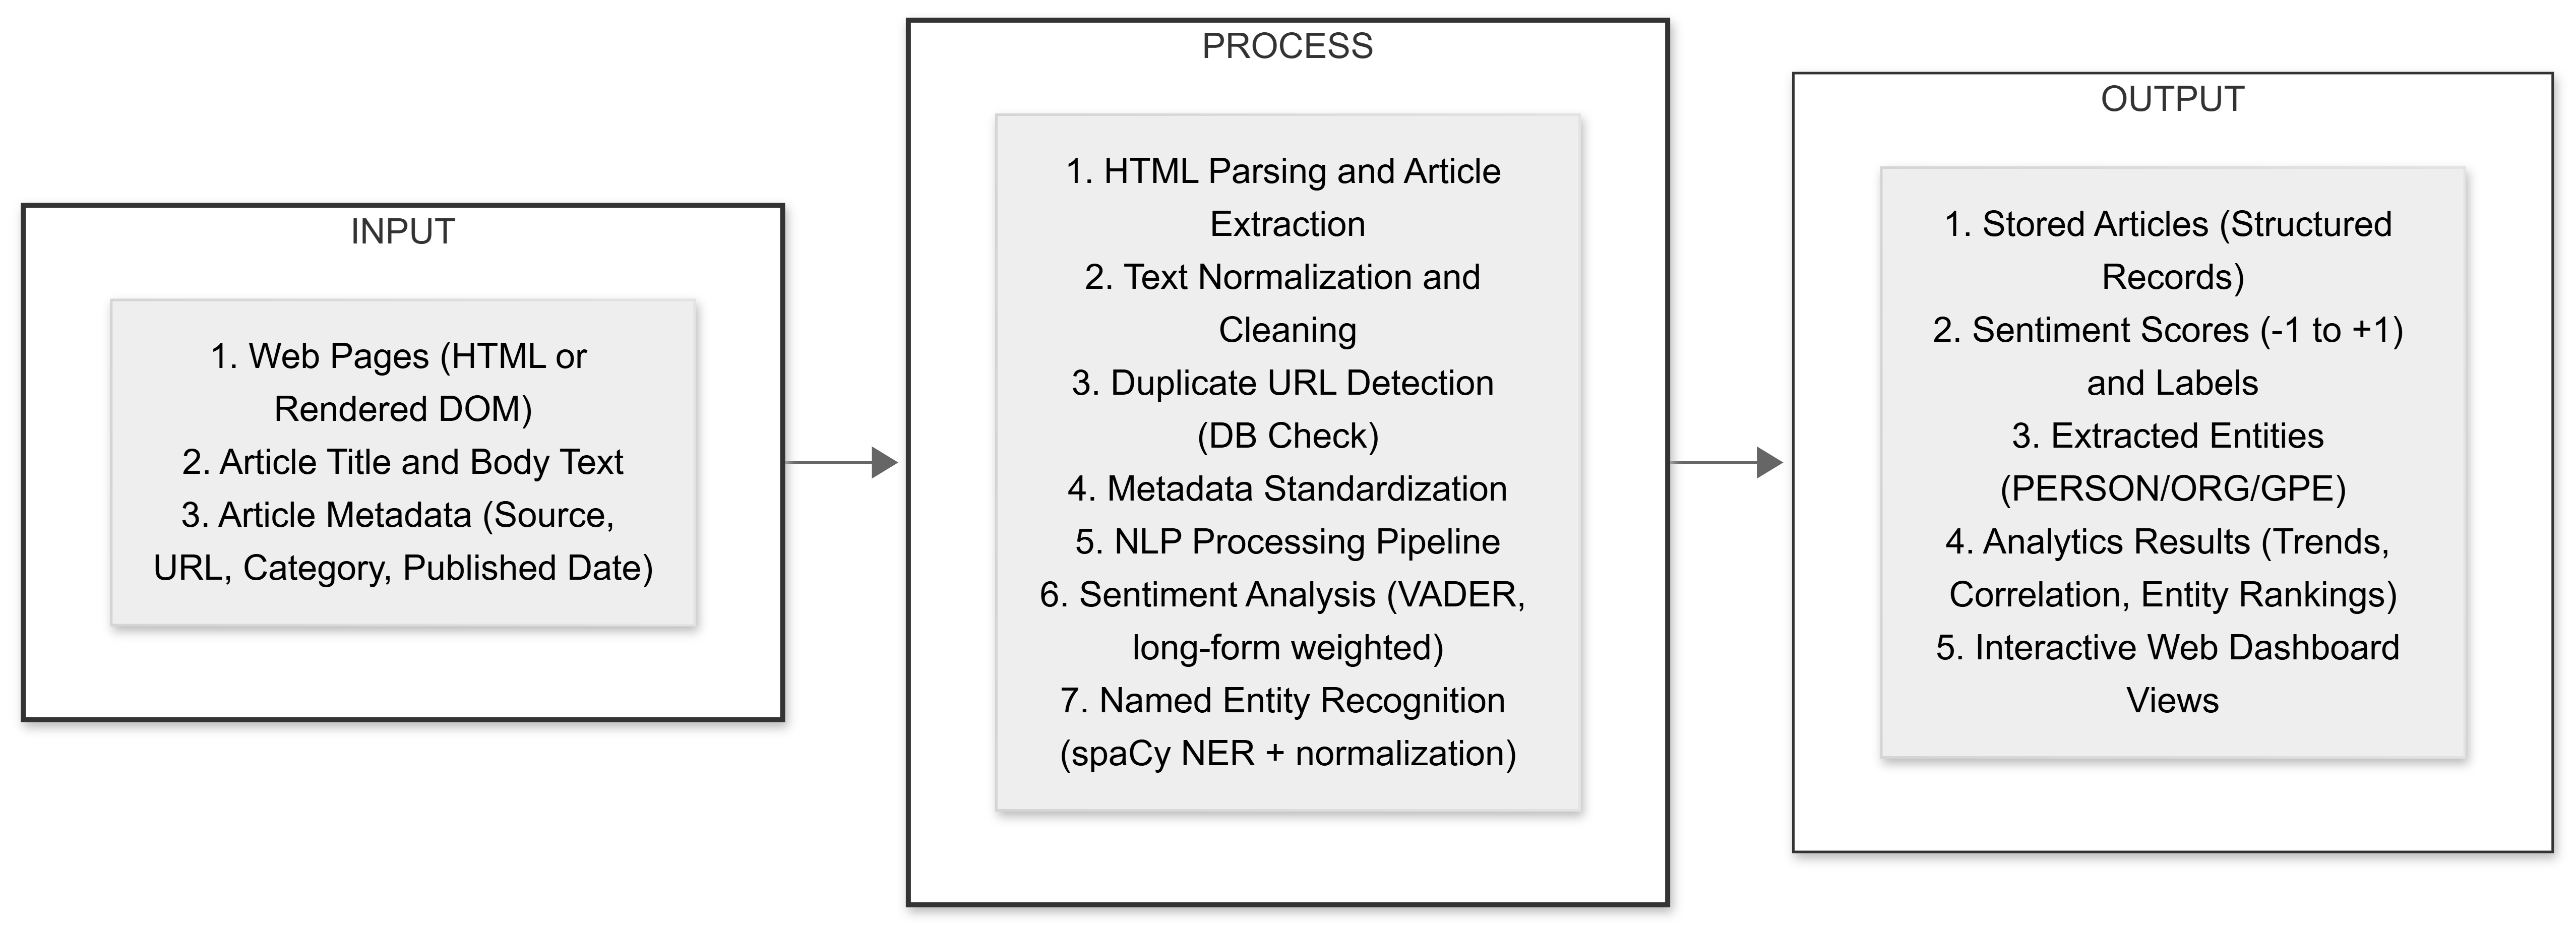
\includegraphics[width=6.26042in,height=2.25in]{docx-media/1ead301e066450bf0471d0c384c81e5c0cd8bb19.png}

\textbf{Figure 1} illustrates the Input--Process--Output (IPO) conceptual framework of the study. This framework describes how raw news data is collected, processed through analytical methods, and transformed into interpretable outputs for media sentiment monitoring.

The \textbf{Input component} consists of news articles collected from seven 6 major Philippine news websites. These inputs include web pages retrieved from the target sources (HTML or rendered page content), extracted article titles and body text, and associated metadata such as publication date, source name, category, and article URL. These materials serve as the primary textual dataset used for analysis.

The \textbf{Process component} represents the analytical pipeline applied to the collected data. First, automated web scraping retrieves article content and metadata from the selected news platforms. Second, data normalization is performed to ensure consistency across different sources. This stage includes text cleaning, metadata standardization, and duplicate URL detection through database checks to prevent redundant records. After preprocessing, Natural Language Processing (NLP) techniques are applied. Sentiment analysis using the VADER model generates polarity scores and sentiment labels, while spaCy's Named Entity Recognition (NER) identifies entities such as persons, organizations, and geographic locations within the news text.

The \textbf{Output component} consists of structured analytical results derived from the processed data. These include sentiment scores ranging from −1.0 to +1.0, categorical sentiment labels (positive, neutral, or negative), extracted named entities, and normalized article records stored in a relational database. These outputs are presented through an interactive analytics dashboard that visualizes sentiment trends, cross-source comparisons, and entity-level summaries, enabling systematic interpretation of media sentiment patterns over time.

\textbf{Scope and Delimitations}

This study focuses exclusively on English-language news articles published by major Philippine national outlets specifically \emph{GMA News Online, Rappler, Inquirer.net, The Manila Times, The Manila Bulletin,} and \emph{The Philippine Star}. Data collection began on \textbf{September 4, 2025}, and continues automatically throughout the study period. For analysis, only articles available up to the point of evaluation are included, providing a snapshot of the dataset at that time.

The analysis is restricted to the textual components of news reports and excludes multimedia elements such as images, videos, advertisements, embedded posts, and comment sections. Opinion pieces, editorials, and satire articles are also excluded to maintain neutrality and minimize subjective author bias.

The study's analytical scope is confined to sentiment polarity and named entity-- sentiment associations. While these associations can reveal emerging trends and potential indicators of media tone or framing bias, the system does not attempt to classify or label such biases directly. Comprehensive bias evaluation remains beyond the present scope and is identified as a potential direction for future research.

These delimitations ensure that the research remains technically feasible, analytically focused, and aligned with its primary objective of identifying sentiment trends and entity-level sentiment patterns across prominent national news sources.

\subsubsection{\texorpdfstring{\textbf{Significance of the Study}}{Significance of the Study}}\label{significance-of-the-study}

This study contributes to the intersection of computational linguistics and media monitoring by providing a scalable framework for the automated analysis of Philippine online news. By implementing a hybrid Natural Language Processing (NLP) pipeline that integrates lexicon-based sentiment analysis {[}8{]} with neural-based entity recognition {[}26{]}, the system enables continuous and structured monitoring of sentiment patterns across digital news sources. This approach establishes a baseline for high-frequency sentiment observation within the Philippine online news ecosystem.

The significance of this work can be observed across several stakeholder groups.

\textbf{Media Organizations and Newsrooms.}

The system provides data-driven indicators that may support the examination of reporting tone across time and across different news outlets. By observing sentiment distributions and entity-level trends, media organizations may explore potential patterns in news coverage and reporting tone without replacing editorial judgment or qualitative analysis.

\textbf{Media Watchdogs and Fact-Checking Institutions (e.g., CMFR, VERA Files).}

Organizations dedicated to media accountability may use automated monitoring tools to complement existing manual review processes. The system can assist in identifying long-term agenda-setting indicators and shifts in media tone that may warrant further investigation through traditional content analysis methods {[}11{]}.

\textbf{The General Public and Digital News Consumers.}

Through interactive sentiment visualizations and aggregated news indicators, the system promotes improved media literacy by enabling readers to observe how emotional tone evolves within news reporting. Presenting large volumes of articles in summarized visual form allows users to interpret news discourse more critically rather than relying solely on individual articles {[}34{]}.

\textbf{Policymakers and Communication Agencies.}

Government communication offices and policy analysts may use aggregated sentiment indicators in news reporting as supplementary signals when examining how policy-related topics are represented in media discourse.

\textbf{Academic Researchers and NLP Practitioners.}

The system also serves as a practical implementation reference for hybrid NLP pipelines applied to real-world media datasets. By integrating technologies such as FastAPI {[}27{]}, Celery {[}29{]}, and Supabase {[}19{]}, the study demonstrates how distributed services can support scalable data collection, processing, and visualization in localized analytical environments.

Overall, this study demonstrates how automated sentiment monitoring can support the systematic observation of media discourse. By providing structured sentiment indicators and entity-level analytics, the system enables exploratory analysis of reporting tone across Philippine digital news sources. More importantly, the study demonstrates the feasibility of applying hybrid Natural Language Processing techniques to monitor sentiment patterns in Philippine online news, providing a practical foundation for future research in computational media analysis within the local media environment.

\subsubsection{\texorpdfstring{\textbf{Definition of Terms}}{Definition of Terms}}\label{definition-of-terms}

To ensure clarity and consistency, the following key terms are defined operationally for the purpose of this study:

\textbf{Natural Language Processing (NLP).}\\
A branch of Artificial Intelligence (AI) that enables computers to analyze and interpret human language in textual form {[}1{]}.

\textbf{Sentiment Analysis.}\\
A Natural Language Processing technique used to computationally identify and categorize the emotional tone expressed in text as positive, neutral, or negative {[}8, 10{]}.

\textbf{Polarity.}\\
The directional orientation of sentiment within a text, typically represented as a numerical score or categorical label indicating positive, neutral, or negative sentiment {[}8{]}.

\textbf{Named Entity Recognition (NER).}\\
A Natural Language Processing method that automatically detects and classifies named entities in text into predefined categories such as persons, organizations, and locations {[}12, 26{]}.

\textbf{Web Scraping.}\\
The automated extraction of structured data from websites using browser automation tools or HTTP requests. In this study, it refers to the collection of news articles from selected Philippine news sources for analysis {[}30{]}.

\textbf{Media Sentiment.}\\
The overall emotional tone conveyed by news content toward specific entities, topics, or events, which may serve as an indicator for exploring patterns in media framing and agenda-setting {[}4, 11{]}.

\textbf{Visualization Dashboard.}\\
A graphical user interface that presents processed analytical data through interactive charts, tables, and visual components to support interpretation of sentiment trends {[}31, 34{]}.

\textbf{Philippine News Media.}\\
Digital news organizations and online publications operating within the Philippines that serve as the primary sources of textual data analyzed in this study {[}3, 17{]}.

\begin{quote}
\textbf{CHAPTER II}

\textbf{Review of Related Literature}
\end{quote}

\textbf{Introduction}

This chapter provides a comprehensive review of theoretical frameworks and empirical studies that are relevant to automated sentiment analysis in Philippine online news media. It begins by discussing foundational theories in communication research, particularly Framing and Agenda-Setting, and their operational relevance to measurable linguistic features. Following this, the chapter examines international computational studies on sentiment analysis and biased language, highlighting methodological developments, practical applications, and limitations. The discussion then moves to local studies in the Philippines, analyzing how these research efforts inform current challenges and gaps. Finally, the chapter reviews major computational methods in sentiment analysis, synthesizes research gaps, emphasizes the conceptual contribution of the present study, and considers ethical and practical implications.

\subsection{\texorpdfstring{\textbf{Theoretical Background}}{Theoretical Background}}\label{theoretical-background}

\subsection{Framing Theory explains that the selection, emphasis, and presentation of textual elements guide audience interpretation by shaping the context in which facts are understood {[}4{]}. Agenda-Setting Theory indicates that the prominence and repetition of topics by mass media influence which issues the public perceives as important {[}11{]}. Both theories foreground salience and valence of media content; in computational terms, these map to measurable features such as frequency, topical prominence, and sentiment polarity.}\label{framing-theory-explains-that-the-selection-emphasis-and-presentation-of-textual-elements-guide-audience-interpretation-by-shaping-the-context-in-which-facts-are-understood-4.-agenda-setting-theory-indicates-that-the-prominence-and-repetition-of-topics-by-mass-media-influence-which-issues-the-public-perceives-as-important-11.-both-theories-foreground-salience-and-valence-of-media-content-in-computational-terms-these-map-to-measurable-features-such-as-frequency-topical-prominence-and-sentiment-polarity.}

From a linguistic-computational perspective, editorial stance is reflected in linguistic devices such as evaluative adjectives, hedging terms, presuppositions, amplifiers, and subjective verbs. These textual signals can be quantified and modeled computationally. Prior work has demonstrated that such cues can be operationalized as feature sets for large-scale bias and subjectivity detection frameworks {[}20{]}.

\subsubsection{\texorpdfstring{\textbf{Operational Link to Computational Measures}}{Operational Link to Computational Measures}}\label{operational-link-to-computational-measures}

\subsubsection{Salience: Topic frequency, headline prominence, and entity mention counts.}\label{salience-topic-frequency-headline-prominence-and-entity-mention-counts.}

\subsubsection{Valence/Tone: Sentence- and document-level sentiment polarity and intensity.}\label{valencetone-sentence--and-document-level-sentiment-polarity-and-intensity.}

\subsubsection{Framing Devices: Lexical features (hedges, presuppositions), syntactic constructions, and discourse markers detected algorithmically.}\label{framing-devices-lexical-features-hedges-presuppositions-syntactic-constructions-and-discourse-markers-detected-algorithmically.}

\subsubsection{This theoretical mapping justifies the use of sentiment analysis and lexical/syntactic signal detection as empirical proxies for framing and agenda-setting phenomena in news media}\label{this-theoretical-mapping-justifies-the-use-of-sentiment-analysis-and-lexicalsyntactic-signal-detection-as-empirical-proxies-for-framing-and-agenda-setting-phenomena-in-news-media}

\section{International Empirical Studies on Sentiment and Biased Language}\label{international-empirical-studies-on-sentiment-and-biased-language}

International scholarship provides the methodological and empirical foundation for understanding how computational systems interpret tone and contextual cues in media. Four major lines of inquiry have emerged:

\subsubsection{\texorpdfstring{\textbf{Lexicon- and Rule-Based Approaches}}{Lexicon- and Rule-Based Approaches}}\label{lexicon--and-rule-based-approaches}

Lexicon- and rule-based approaches remain influential due to their interpretability. Through extensive validation, the VADER framework was shown to reliably capture polarity and intensification, establishing it as a practical baseline for high-volume environments {[}8{]}.

\subsubsection{\texorpdfstring{\textbf{Machine Learning and Transformer Approaches}}{Machine Learning and Transformer Approaches}}\label{machine-learning-and-transformer-approaches}

Subsequent studies expanded sentiment analysis through deep-learning architectures. Transformer-based systems such as BERT and RoBERTa significantly outperform traditional classifiers in detecting nuanced sentiment but present challenges regarding computational cost and domain-specific shifts {[}10, 14{]}.

\subsubsection{\texorpdfstring{\textbf{Hybrid Approaches}}{Hybrid Approaches}}\label{hybrid-approaches}

Combining lexicon-based features with supervised machine-learning improves robustness in noisy and informal text domains {[}9{]}.

\subsubsection{\texorpdfstring{\textbf{Targeted / Entity-Level Sentiment Analysis}}{Targeted / Entity-Level Sentiment Analysis}}\label{targeted-entity-level-sentiment-analysis}

Recent work emphasizes targeted sentiment analysis, associating polarity with specific actors or institutions rather than assigning a single score to a document {[}12{]}.

Recent syntheses by Leon {[}10{]} and Rana {[}14{]} clarify the evolution from rule-based heuristics to neural architectures. Leon {[}10{]} argues that while the shift to Transformers represents a paradigm change in accuracy, systems must reconcile the transparency of earlier lexicon models with the predictive power of modern architectures. Similarly, Rana {[}14{]} highlights that Transformer-based models are superior in capturing nuanced emotional cues and sarcasm that traditional lexicons often misinterpret. These reviews justify the multi-model approach of the present study, balancing high-speed lexicon processing with the deep contextual understanding of modern pipelines.

\section{Local (Philippine) Studies}\label{local-philippine-studies}

Research on sentiment analysis and Natural Language Processing (NLP) in the Philippines has expanded, yet studies face limitations in scale and automation.

\subsubsection{\texorpdfstring{\textbf{Sentiment of Newspaper Headlines}}{Sentiment of Newspaper Headlines}}\label{sentiment-of-newspaper-headlines}

Diaz {[}3{]} examined headlines from major Philippine broadsheets, finding that most exhibited negative sentiment, suggesting emotionally charged framing aimed at capturing attention. While insightful, the manual sampling design and focus on headlines rather than full articles prevented continuous analysis.

\subsubsection{\texorpdfstring{\textbf{COVID-19 Sentiment in Metro Manila}}{COVID-19 Sentiment in Metro Manila}}\label{covid-19-sentiment-in-metro-manila}

Complementing news-centric studies, Garcia {[}5{]} analyzed the emotional landscape of Metro Manila during the COVID-19 pandemic through social media. This study demonstrated how computational tools could track public anxiety in response to policy shifts, though it highlighted the difficulty of analyzing Philippine-specific contexts using generic tools.

\subsubsection{\texorpdfstring{\textbf{Fake News and Economic Monitoring}}{Fake News and Economic Monitoring}}\label{fake-news-and-economic-monitoring}

Other local research investigated fake news classification, finding that sentiment features can assist in distinguishing stylistic differences across sources {[}23{]}. Furthermore, the Bangko Sentral ng Pilipinas developed high-frequency News Sentiment Indices that correlated strongly with economic indicators, demonstrating the value of media sentiment as a macroeconomic signal {[}22{]}.

\subsubsection{\texorpdfstring{\textbf{Institutional and Structural Monitoring}}{Institutional and Structural Monitoring}}\label{institutional-and-structural-monitoring}

Studies by the Philippine Institute for Development Studies {[}25{]} revealed divergent sentiment patterns toward government policies, while the Center for Media Freedom and Responsibility {[}17{]} provided insights into issue salience during election cycles through human coding. Finally, the Media Ownership Monitor Philippines {[}24{]} investigates structural media conditions but is updated only at multi-year intervals.

\subsubsection{\texorpdfstring{\textbf{Philippine NLP Baselines}}{Philippine NLP Baselines}}\label{philippine-nlp-baselines}

A technical foundation for localized automation is provided by Cruz and Cheng {[}2{]}, who established baseline performance metrics for text classification in Filipino. Their work demonstrated that fine-tuning pre-trained Transformer models on local datasets significantly outperforms traditional machine learning for Philippine text, providing the justification for utilizing advanced architectures to handle unique syntax and code-switching in local news.

\subsubsection{\texorpdfstring{\textbf{Methods-in-the-Literature}}{Methods-in-the-Literature}}\label{methods-in-the-literature}

\subsubsection{This subsection surveys commonly used methodological approaches and summarises their strengths and weaknesses as found in the literature. The objective here is to situate the methodological landscape informing method choice.}\label{this-subsection-surveys-commonly-used-methodological-approaches-and-summarises-their-strengths-and-weaknesses-as-found-in-the-literature.-the-objective-here-is-to-situate-the-methodological-landscape-informing-method-choice.}

{\def\LTcaptype{none} % do not increment counter
\begin{longtable}[]{@{}
  >{\raggedright\arraybackslash}p{(\linewidth - 6\tabcolsep) * \real{0.2588}}
  >{\raggedright\arraybackslash}p{(\linewidth - 6\tabcolsep) * \real{0.2048}}
  >{\raggedright\arraybackslash}p{(\linewidth - 6\tabcolsep) * \real{0.2566}}
  >{\raggedright\arraybackslash}p{(\linewidth - 6\tabcolsep) * \real{0.2799}}@{}}
\toprule\noalign{}
\begin{minipage}[b]{\linewidth}\raggedright
\textbf{Method/Component}
\end{minipage} & \begin{minipage}[b]{\linewidth}\raggedright
\textbf{Typical Use Cases}
\end{minipage} & \begin{minipage}[b]{\linewidth}\raggedright
\textbf{Main Advantages}
\end{minipage} & \begin{minipage}[b]{\linewidth}\raggedright
\textbf{Main Limitation}
\end{minipage} \\
\midrule\noalign{}
\endhead
\bottomrule\noalign{}
\endlastfoot
\textbf{Lexicon / Rule-based (e.g., VADER)} & Social media, news headlines & Fast, interpretable, low latency & Domain mismatch, sarcasm {[}8{]} \\
\textbf{Transformer models (BERT)} & High-accuracy tasks & Strong contextual understanding & High compute cost, domain-shift {[}10, 14{]} \\
\textbf{Hybrid Pipelines} & Noisy domains, limited data & Production-ready, robust & Pipeline complexity {[}9{]} \\
\textbf{NER Tools (spaCy)} & Entity-level mapping & Balances performance/interpretability & Requires domain adaptation {[}12, 26{]} \\
\end{longtable}
}

By reviewing these methods, the literature reveals trade-offs between accuracy and speed, interpretability and black-box complexity, and flexibility versus maintenance under domain shift. These trade-offs inform methodological decisions in the present study.

\textbf{Synthesis: Research Gaps and Conceptual Contribution}

Three key insights emerge from the reviewed literature. First, international research demonstrates methodological trade-offs: transformer models offer accuracy but require extensive resources, while lexicon-based approaches remain valuable for real-time monitoring {[}8, 10, 14{]}. Second, local Philippine studies are limited in automation, temporal coverage, and scale {[}3, 23, 25{]}. Third, a design opportunity exists: efficient lexicon-based sentiment analyzers, complemented by entity recognition, provide a practical foundation for scalable, continuous media analytics. These insights collectively establish the rationale for the present study, which aims to implement an automated, multi-source, temporally adaptive system for Philippine news media monitoring.

\textbf{Ethical and Practical Considerations}

Real-time sentiment monitoring introduces both methodological and ethical challenges. Lexicon-based models may misinterpret nuanced language, including sarcasm or contextual framing. Therefore, sentiment scores in this study are treated as indicative signals rather than definitive judgments. This approach balances interpretability, timeliness, and computational efficiency while acknowledging limitations inherent to automated analysis. Future research may enhance fidelity by integrating hybrid or transformer-based models.

\begin{quote}
\textbf{CHAPTER III}
\end{quote}

\section{\texorpdfstring{\textbf{Technicality of the Project}}{Technicality of the Project}}\label{technicality-of-the-project}

The technical complexity of \emph{Sentiment Analysis of Philippine Media News Using Natural Language Processing} lies in the development of an automated, end-to-end data processing pipeline capable of continuously collecting, analyzing, and presenting insights from dynamically generated online news content. The system integrates web automation, distributed task processing, natural language processing (NLP), and interactive data visualization within a modular, service-oriented architecture. Through the coordination of these components, unstructured web-based news articles are transformed into structured analytical outputs that can be used for sentiment monitoring and media analysis.

Unlike traditional static websites, many modern news platforms including Rappler and GMA News rely heavily on JavaScript-driven page rendering. In such environments, the content visible to users is generated dynamically after the initial page load. As a result, conventional scraping methods based solely on HTTP requests and HTML parsing are often insufficient for extracting complete article information. To address this limitation, the project utilizes headless browser automation tools that simulate real user interaction with the webpage, allowing scripts and dynamic elements to fully render before the extraction process begins. This approach significantly improves the reliability and completeness of the collected news data {[}30{]}.

Another technical challenge arises from the computational requirements of natural language processing. Tasks such as sentiment scoring, entity recognition, and text preprocessing can introduce significant latency when executed directly within a synchronous application workflow. If these operations are handled within the main request--response cycle of the system, they may slow down the overall performance of the application. To mitigate this issue, the project adopts a distributed task processing architecture that separates data acquisition from analytical computation. Scraping tasks and NLP operations are delegated to background workers, enabling asynchronous processing that allows the system to continue collecting data while analytical computations are performed independently {[}29{]}.

The project also employs a hybrid computational linguistics framework that integrates lexicon-based sentiment analysis with neural Named Entity Recognition. Lexicon-based sentiment scoring, implemented through the VADER model, provides interpretable polarity scores for textual content by evaluating the presence and intensity of sentiment-bearing words {[}8{]}. At the same time, Named Entity Recognition models are used to identify important entities such as persons, organizations, and locations within news articles, providing additional contextual information about the content being analyzed {[}26{]}. The combination of these approaches allows the system to generate richer analytical outputs that include both emotional polarity and structural entity information.

Overall, the technical complexity of the project lies not in a single algorithm but in the coordination of multiple subsystems responsible for data acquisition, processing, storage, and presentation. These subsystems operate together to transform large volumes of unstructured news data into structured insights suitable for monitoring sentiment trends and analyzing media narratives.

\paragraph{\texorpdfstring{\textbf{Details of the Technologies to be Used}}{Details of the Technologies to be Used}}\label{details-of-the-technologies-to-be-used}

The system adopts a modern technology stack designed to support scalability, modularity, and efficient data processing. Each component of the architecture addresses a specific responsibility within the pipeline, including web data acquisition, backend service management, distributed computation, natural language processing, data storage, and user-facing visualization.

\textbf{Web Data Acquisition}

The project uses Playwright {[}30{]}, a headless browser automation framework, to extract data from JavaScript-driven news platforms. Playwright enables full browser rendering before content extraction, ensuring accurate retrieval of complete articles.

\textbf{Backend Service Architecture}

The backend is implemented using FastAPI {[}27{]}, a high-performance Python web framework optimized for asynchronous operations. The backend follows RESTful architectural principles, using Uvicorn {[}28\textbf{{]}} as the ASGI server. This design cleanly separates internal data processing services from the user-facing frontend.

\textbf{Distributed Task Processing}

To prevent computational bottlenecks, the system employs Celery {[}29{]} as a distributed task queue, with Redis {[}15{]} acting as the message broker and result backend. Celery enables asynchronous execution of scraping and NLP-related tasks independent of the main API process. Redis functions as a lightweight, in-memory data store that manages task queues and intermediate results efficiently {[}15{]}.

\textbf{Natural Language Processing Framework}

The NLP layer combines two complementary tools:

\begin{enumerate}
\def\labelenumi{\arabic{enumi}.}
\item
  Lexicon-based sentiment analysis: Utilizing the VADER framework {[}8{]} for computing polarity scores over article text. VADER is specifically tuned for sentiment expression in social and news media {[}8{]}.
\item
  spaCy {[}26{]}: Used for Named Entity Recognition (NER), specifically identifying persons, organizations, and locations within news articles.
\end{enumerate}

\textbf{Data Storage and Persistence}

The system uses PostgreSQL {[}6{]}, provisioned through Supabase {[}19{]}, as its primary relational database. PostgreSQL ensures reliability and strong ACID guarantees for article metadata and analytical results {[}6{]}. Additionally, the analysis pipeline utilizes NumPy {[}7{]}, SciPy {[}20{]}, Scikit-learn {[}13{]}, and pandas {[}36{]} for structured data manipulation and fundamental algorithms {[}20, 36{]}.

\textbf{Frontend Analytical Interface}

The frontend is developed using Next.js {[}31{]}, React {[}32{]}, and TypeScript, providing a responsive analytics dashboard. For visualization, the system uses Recharts {[}34{]} to render sentiment timelines and source comparisons. Tailwind CSS {[}33{]} is used for utility-first styling

\textbf{Technology Stack Justification}

The overall technology stack was selected to support several key system requirements, including scalability, modularity, performance efficiency, and maintainability.

{\def\LTcaptype{none} % do not increment counter
\begin{longtable}[]{@{}
  >{\raggedright\arraybackslash}p{(\linewidth - 4\tabcolsep) * \real{0.1145}}
  >{\raggedright\arraybackslash}p{(\linewidth - 4\tabcolsep) * \real{0.3048}}
  >{\raggedright\arraybackslash}p{(\linewidth - 4\tabcolsep) * \real{0.5807}}@{}}
\toprule\noalign{}
\begin{minipage}[b]{\linewidth}\raggedright
\textbf{Goal}
\end{minipage} & \begin{minipage}[b]{\linewidth}\raggedright
\textbf{Technologies Used}
\end{minipage} & \begin{minipage}[b]{\linewidth}\raggedright
\textbf{Justification}
\end{minipage} \\
\midrule\noalign{}
\endhead
\bottomrule\noalign{}
\endlastfoot
\textbf{Scalability} & Celery {[}29{]}, Redis {[}15{]}, FastAPI {[}27{]} & Handles concurrent dashboard requests and async background tasks. \\
\textbf{Modularity} & Supabase {[}19{]}, Next.js {[}31{]} & Clear separation of persistence, API, and presentation layers. \\
\textbf{Performance} & Playwright {[}30{]}, Redis {[}15{]} & Enables non-blocking operations and efficient data caching. \\
\textbf{Reliability} & PostgreSQL {[}6{]}, Docker {[}35{]} & Ensures data integrity and consistent deployment environments {[}35{]}. \\
\end{longtable}
}

Collectively, these technologies allow the system to handle continuously updating online news content while maintaining analytical responsiveness, structural stability, and a clean separation of concerns that is appropriate for a production‑style capstone project.

\begin{quote}
\textbf{CHAPTER IV}
\end{quote}

\textbf{METHODOLOGY}

This chapter presents the methodology adopted in the analysis, design, and development of the proposed PH Eye: Automated Media Sentiment Monitoring System for Philippine online news platforms. It outlines the structured approach used to translate system requirements into functional models, architectural designs, and operational components necessary for the implementation of the system.

The chapter begins with requirements modeling, which identifies and defines the functional and non-functional requirements that guide the development of the system. These requirements establish the system's core capabilities, including automated data collection from online news platforms, sentiment analysis, entity extraction, and visualization of analytical results.

Following the requirements analysis, the chapter discusses data and process modeling, which describes how information flows throughout the system. This section presents several modeling tools, including the context diagram, data flow diagrams (DFD), system flowcharts, and program flowcharts, which collectively illustrate how data is captured, processed, and transformed within the system.

The chapter then presents the system design, which includes the output design and user-interface design, detailing the forms and reports generated by the system. In addition, the logical structure of the system's database is described through the Entity Relationship Diagram (ERD), which defines the relationships among the major data entities used in the application.

Subsequently, the development section outlines the technical environment used in implementing the system. This includes the software specifications, hardware requirements, program structure, and the programming environment used during development, including both the frontend and backend components of the system.

Finally, the chapter presents an overview of the system architecture, describing how the major components of the application interact to support automated data acquisition, processing, storage, and visualization. Through this methodology, the study ensures that the system is systematically designed, technically sound, and aligned with the objectives of automated sentiment analysis {[}8{]} and named entity extraction {[}26{]} for Philippine digital news platforms.

\subsubsection{\texorpdfstring{\textbf{Software Development Life Cycle (SDLC)}}{Software Development Life Cycle (SDLC)}}\label{software-development-life-cycle-sdlc}

This study adopted an \textbf{Iterative Software Development Life Cycle (SDLC) model}. The iterative approach was selected because the system required continuous refinement, frequent testing, and rapid adaptation to issues commonly encountered in web scraping, data preprocessing, and Natural Language Processing (NLP) workflows.

The SDLC guided the technical development of the system, while the research design guided the analytical component of the study. Under this approach, the system was developed through repeated development cycles, where each cycle produced a functional subsystem that was tested and refined in subsequent iterations.

Through this iterative process, major components such as the scraping pipeline, text preprocessing module, sentiment analysis engine, API backend, and interactive dashboard were progressively implemented and improved. Each iteration allowed the system to be evaluated using real-world data, enabling adjustments to scraping strategies, NLP parameters, and database workflows.

This development strategy enhanced system reliability and ensured that the platform remained stable despite variations in website structure, article formatting, and incoming data characteristics.

\textbf{Figure 4.0 Iterative Software Development Life Cycle for the Automated Media Sentiment Monitoring System}

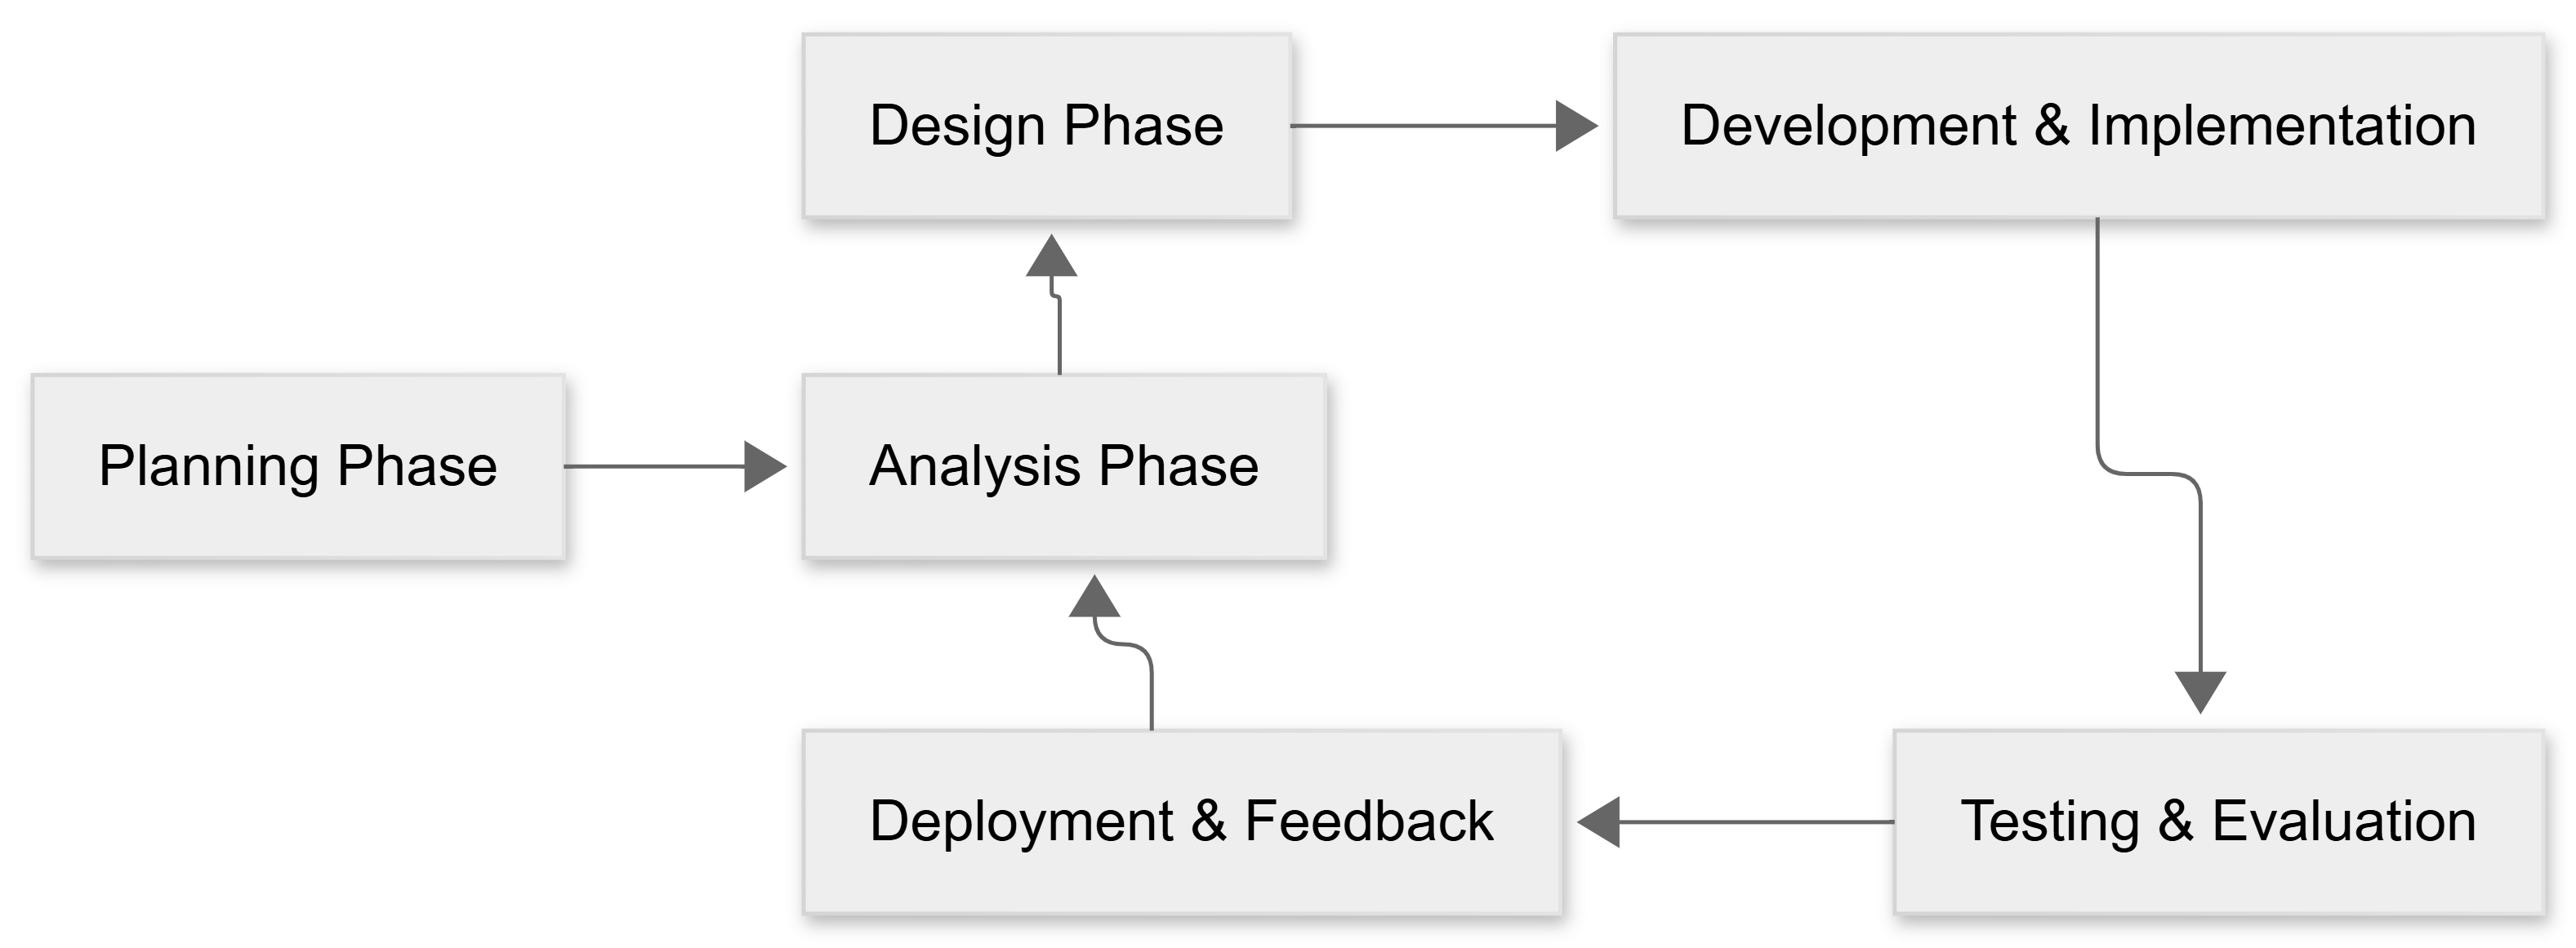
\includegraphics[width=6.26042in,height=2.30208in]{docx-media/a1ebcc2569e7562cab70ab51e3dac213822da673.png}

The implemented system follows an \textbf{iterative Software Development Life Cycle (SDLC)}, as depicted in \textbf{Figure 4.0.} This model was chosen because the system involves continuously changing online news sources, requiring frequent adaptation and refinement of the scraping, natural language processing, and dashboard modules.

\textbf{Planning Phase:} The overall objectives, project scope, and system constraints were defined. Key functional requirements, such as automated article collection, sentiment analysis, entity extraction, and interactive dashboards, were established. Initial planning was performed at project start; subsequent iterations included lightweight iteration planning based on observed system outputs

\textbf{Analysis Phase:} Each iteration begins with a detailed examination of the system's performance and operational results from the previous cycle. This includes verifying scraper effectiveness against website layout changes, checking sentiment behavior and performing evaluation comparisons on recent article samples

\textbf{Design Phase:} Based on the analysis, design decisions are made for the next iteration. This includes refining module interactions, database schemas, API logic, and visualization layouts.

\textbf{Development \& Implementation Phase:} The system is incrementally built, implementing the modules identified in the design phase. Major components include web scrapers, preprocessing pipelines, VADER-based sentiment scoring, spaCy entity extraction, database/API integration, and the frontend dashboard.

\textbf{Testing \& Evaluation Phase:} Each iteration undergoes unit, integration, and end-to-end testing. This ensures that new or refined modules perform correctly and reliably under real-world conditions.

\textbf{Deployment \& Feedback Phase:} The latest system iteration is deployed, and results are monitored. Feedback from deployment informs the next \textbf{Analysis Phase}, enabling continuous improvement while keeping the system aligned with the initial project objectives.

This iterative loop allows the system to evolve gradually, addressing issues as they arise and refining modules incrementally, which is particularly suitable for dynamic environments like online news monitoring.

\subsubsection{\texorpdfstring{\textbf{Requirements Modeling}}{Requirements Modeling}}\label{requirements-modeling}

The requirements for the system are divided into functional requirements, which define what the system must do, and non-functional requirements, which specify the performance and quality attributes of the system.

\paragraph{\texorpdfstring{\textbf{Requirements Modeling}}{Requirements Modeling}}\label{requirements-modeling-1}

The requirements are divided into functional requirements (core actions) and non-functional requirements (performance and quality attributes).

\textbf{Functional Requirements}

Automated Web Scraping: Automatically extract articles from six (6) Philippine news outlets (GMA, Rappler, Inquirer, Philstar, Manila Bulletin, and Manila Times) using Playwright {[}30{]}at scheduled intervals {[}15, 29{]}.

Data Normalization: Clean extracted text using BeautifulSoup4 and NLTK {[}39, 1{]} to remove HTML and whitespace.

Duplicate Detection: Check for existing URLs to prevent redundant processing.

Sentiment Polarity Scoring: Utilize the VADER {[}8{]} tool to assign positive, negative, and neutral scores.

Named Entity Recognition (NER): Utilize spaCy {[}26{]} to identify Persons (PER), Organizations (ORG), and Locations (LOC).

Data Visualization: Provide a dashboard for sentiment trends and entity frequencies using Tailwind CSS and Recharts {[}34, 33{]}.

\textbf{Non-Functional Requirements}

\begin{enumerate}
\def\labelenumi{\arabic{enumi}.}
\item
  Efficiency: Processing pipeline must complete within 60 seconds per article.
\item
  Scalability: Backend architecture (FastAPI {[}27{]} and Celery {[}29{]}) must support adding news sources without significant code changes.
\item
  Reliability: Use Redis {[}15{]} as a message broker to ensure task persistence.
\item
  Usability: The web dashboard must be intuitive, with a responsive design using Next.js,Tailwind and Recharts {[}32, 33, 34{]} that allows users to view data on both desktop and mobile devices.
\item
  Data Integrity: Ensure foreign key constraints in the PostgreSQL {[}6{]} database.
\end{enumerate}

\textbf{Data and Process Modeling}

\emph{\textbf{Context Diagram}}

\textbf{Figure 4.1 Context Diagram of the PH Eye News Sentiment Analysis System}

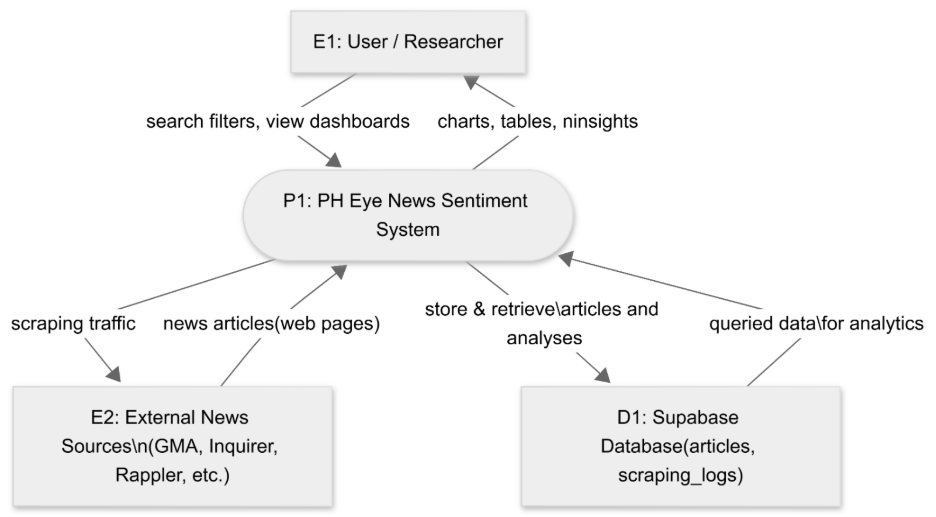
\includegraphics[width=6.5in,height=3.59375in]{docx-media/06431d36391a85f35802309995f8bb6882d37913.png} \textbf{Figure 4.0} shows the Context Diagram of the PH Eye News Sentiment System\textbf{.} It illustrates the system boundary between the central PH Eye web application and its two primary external entities: the User/Researcher and the External News Sources (e.g., GMA, Inquirer, Rappler). Raw news articles are ingested as web pages from these outlets into the PH Eye system, which in turn stores processed articles and analysis results in the Supabase database and delivers summarized charts, tables, and insights back to the user through the web dashboard.

\emph{\textbf{Data Flow Diagram}}

\textbf{Figure 4.2 Data Flow Diagram of the PH Eye News Sentiment Analysis System}

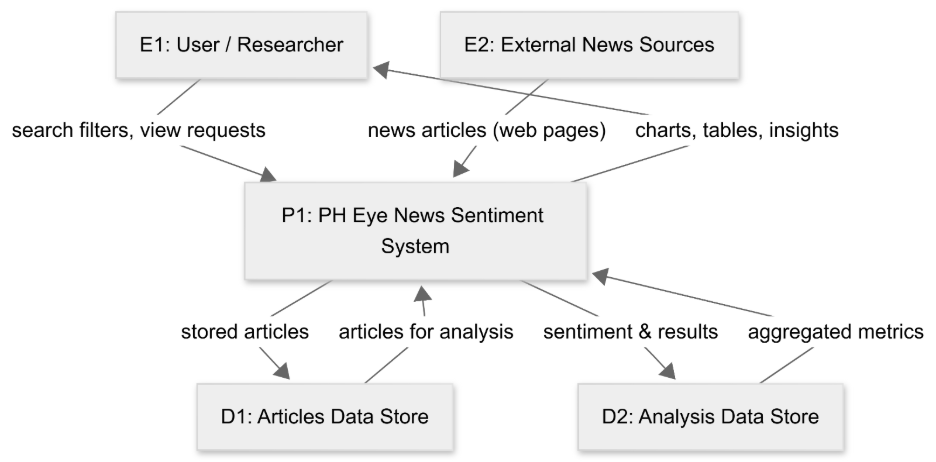
\includegraphics[width=6.5in,height=3.20833in]{docx-media/631af5c051803f3800f4a7be91716e2d6d158652.png} \textbf{Figure 4.2} depicts the core movement of data within the PH Eye system\textbf{.} It shows how incoming news content is transformed from unstructured web pages into structured article records in the Articles Data Store (D1), and how these records are subsequently enriched with sentiment outputs in the Analysis Data Store (D2). The same diagram also highlights how the system reads from these data stores to compute aggregated metrics, which are then returned to the user interface as interpretable insights.

\emph{\textbf{System Flowchart}}

\textbf{Figure 4.3 System Flowchart of the PH Eye News Sentiment Analysis System}

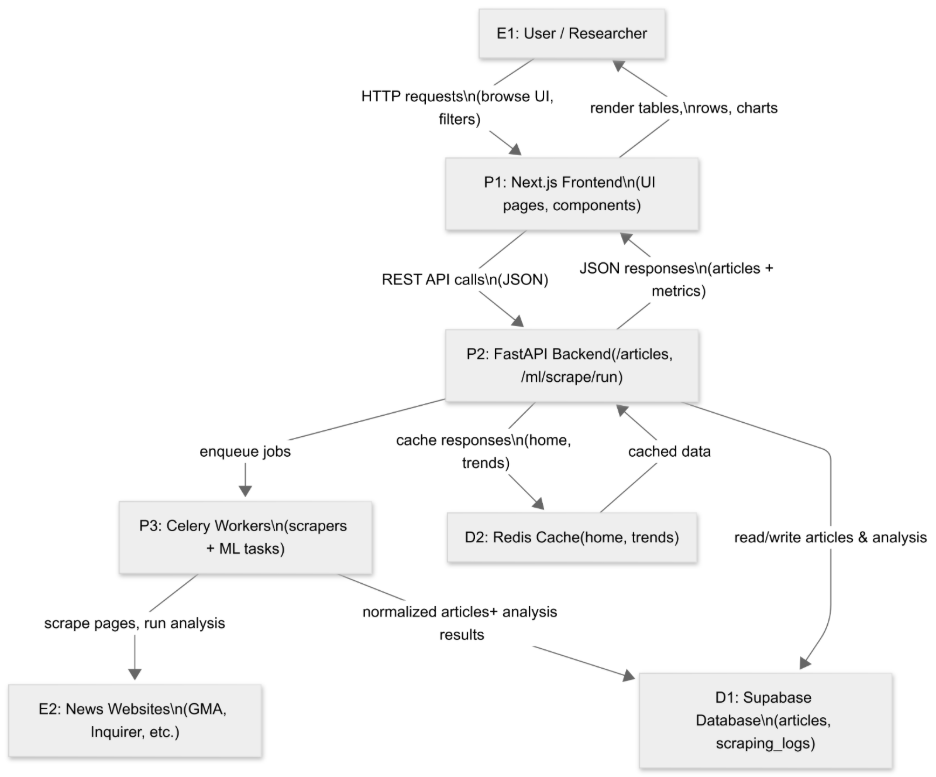
\includegraphics[width=6.5in,height=5.39583in]{docx-media/813c2ce7fb401b686d6c7d47e24a0c64e0df70a6.png} \textbf{Figure 4.3} presents the System Flowchart, which outlines the interaction of the main technical components. The sequence begins when the user issues requests via the Next.js {[}31{]} frontend (P1), which forwards them as API calls to the FastAPI {[}27{]} backend (P2). The backend enqueues scraping and analysis jobs to Celery workers {[}29{]} (P3), which contact external news websites, normalize the articles, and save both raw and analyzed data into Supabase {[}19{]} (D1), while Redis {[}15{]} (D2) is used to cache frequently accessed home, trends, and bias views. Finally, the backend responds with JSON payloads that the frontend renders into up-to-date dashboards for the user.

\emph{\textbf{Program Flowchart}}

\textbf{Figure 4.4 Program flow chart of the PH Eye News Sentiment Analysis System}

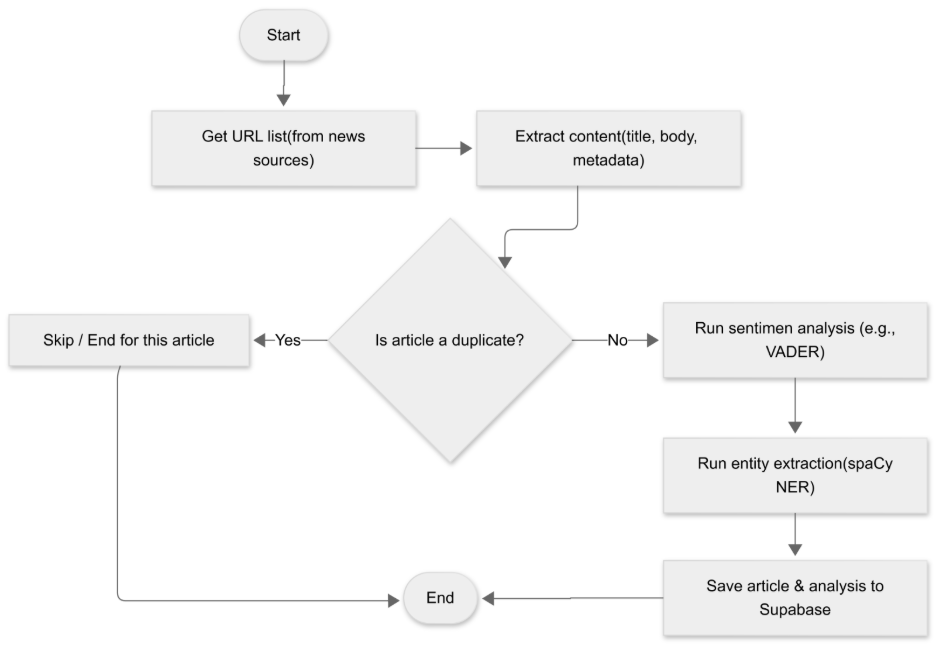
\includegraphics[width=6.5in,height=4.47917in]{docx-media/16fabb1fb715e9dbb3b42fbda3eca67744b21ff2.png}

\textbf{Figure 4.4} describes the high-level logic of the article processing pipeline\textbf{.} For each news URL, the system extracts the article content and then evaluates a decision point to determine whether the article is a duplicate. If it is identified as a duplicate, the flow skips further processing for that item; otherwise, the article passes through sentiment analysis and entity extraction steps (e.g., using VADER-style {[}8{]} sentiment and spaCy-based NER {[}26{]} in the actual implementation). The resulting article and its associated analysis are then stored in Supabase {[}19{]}, completing one iteration of the processing loop.

\subsubsection{\texorpdfstring{\textbf{Design}}{Design}}\label{design}

This section presents the design of the proposed system in terms of user-facing outputs and internal data structures. It first describes the primary interface forms and analytical reports available in the web application, then outlines the logical data model implemented in PostgreSQL (Supabase).

\subsubsection{\texorpdfstring{\textbf{Output and User‑Interface Design}}{Output and User‑Interface Design}}\label{output-and-userinterface-design}

\subsubsection{The output and user-interface design defines how processed analytical results are presented to users. The interface was designed to support exploratory analysis of media sentiment patterns through dashboards, trend visualizations, statistical reports, and searchable article archives. The following forms and reports constitute the primary interaction points of the system.}\label{the-output-and-user-interface-design-defines-how-processed-analytical-results-are-presented-to-users.-the-interface-was-designed-to-support-exploratory-analysis-of-media-sentiment-patterns-through-dashboards-trend-visualizations-statistical-reports-and-searchable-article-archives.-the-following-forms-and-reports-constitute-the-primary-interaction-points-of-the-system.}

\paragraph{\texorpdfstring{\textbf{Forms}}{Forms}}\label{forms}

\section{\texorpdfstring{\textbf{News Dashboard (Home Screen)}}{News Dashboard (Home Screen)}}\label{news-dashboard-home-screen}

The main dashboard displays recently scraped articles grouped by source (GMA, Rappler, Inquirer, Manila Times, Philstar, Sunstar, and Manila Bulletin). Each source block presents article cards containing the headline, publication date, and sentiment label. A View All action per source opens a dedicated source-specific listing for deeper browsing. This layout supports quick cross-source monitoring while preserving organized presentation.

\textbf{Figure 4.5 Homepage of collected articles}

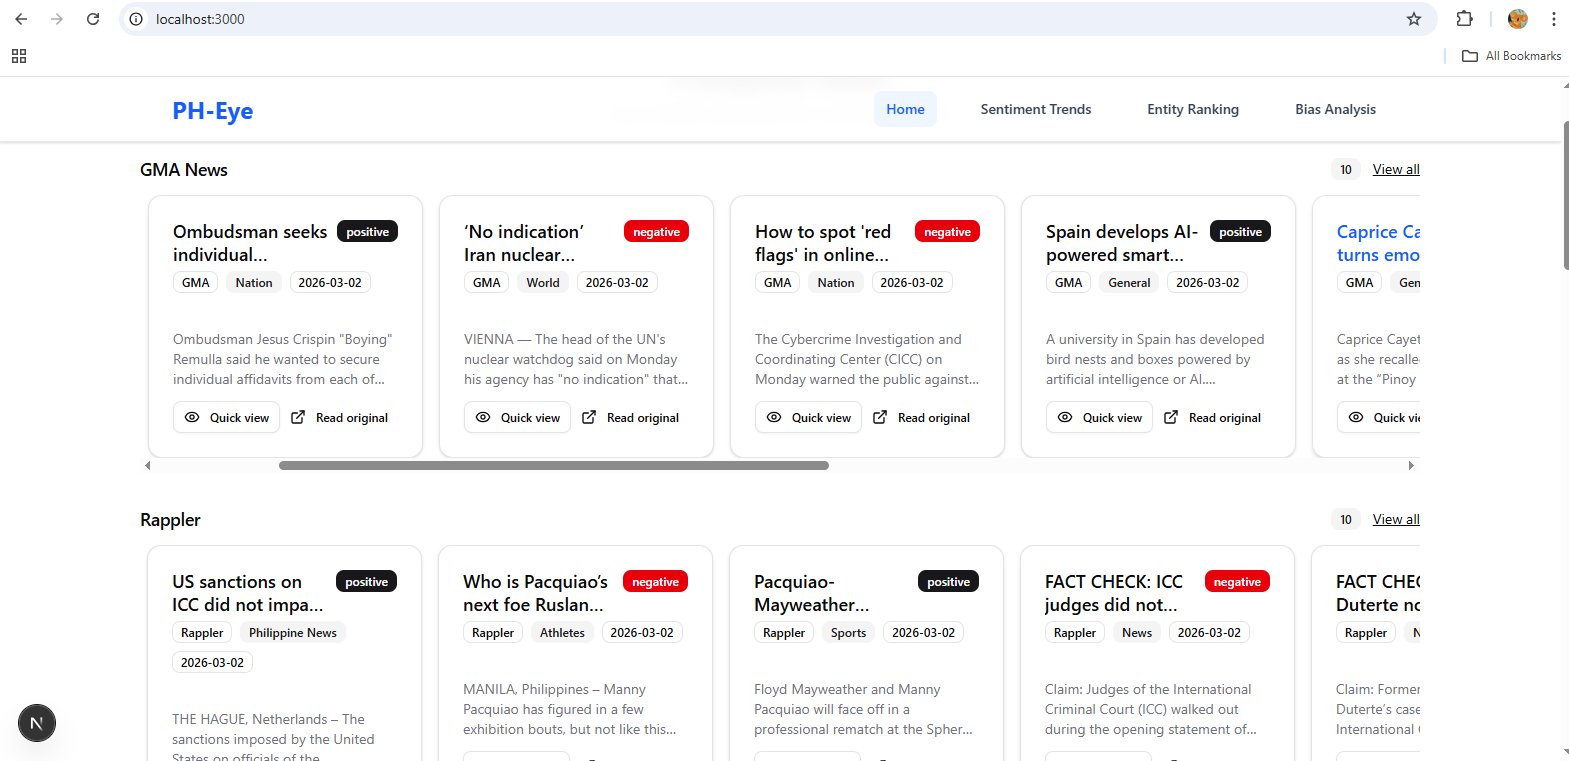
\includegraphics[width=6.26042in,height=3.03125in]{docx-media/9dd112a5568bc177d236b4b6b66f3b88b4c00e97.png}

\textbf{Sentiment Trends Screen}

The Sentiment Trends screen provides interactive filtering controls that allow users to refine the dataset by news source and time period (e.g., last 7 days or last 30 days). The system visualizes sentiment patterns using line charts and summary metrics derived from the stored sentiment analysis results. These visual representations help users identify shifts in public tone and media sentiment over time. The screen is designed to support analytical exploration and trend monitoring.

\textbf{Figure 4.6 Weekly Sentiment Trends}

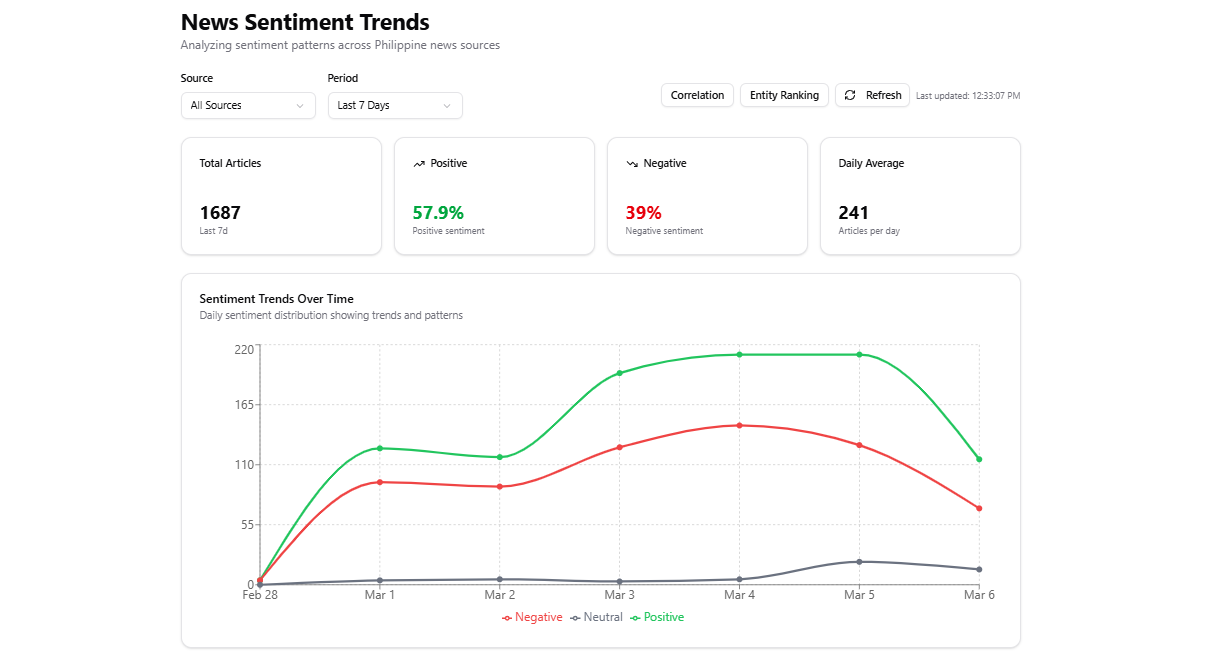
\includegraphics[width=6.26042in,height=3.36458in]{docx-media/05ea950e63338dcc8b9c67bd0e5ce72f2a492634.png}

As shown in \textbf{Figure 4.6}, the Sentiment Trends screen visualizes the daily distribution of positive, neutral, and negative news sentiment across all collected Philippine news sources over a seven-day period. The line chart illustrates how sentiment classifications generated by the VADER sentiment analyzer fluctuate over time.

During the observation window, \textbf{positive sentiment} consistently dominates the dataset, representing approximately \textbf{57.9\%} of the analyzed articles, while \textbf{negative sentiment} accounts for \textbf{39\%} and \textbf{neutral sentiment remains minimal}. The trend lines show a gradual increase in article volume from \textbf{March 1 to March 5}, with positive sentiment maintaining the highest count throughout the period.

The chart also reveals how sentiment levels fluctuate alongside article publication volume. For example, a noticeable increase in both positive and negative articles occurs between \textbf{March 3 and March 5}, corresponding to the period with the highest number of collected articles. This pattern suggests that the sentiment distribution largely reflects the intensity of news coverage during those days.

It is important to note that \textbf{February 28} contains only a small number of collected articles, as the scraper was not executed during part of the data collection period. Consequently, the sentiment distribution on that date should be interpreted cautiously. Despite this limitation, the overall trend still demonstrates the system's ability to track daily sentiment dynamics across multiple Philippine news outlets.

The Sentiment Trends module provides a temporal overview of how media sentiment evolves over time, enabling researchers to identify fluctuations in tone and potential correlations with major news events or reporting cycles.

\textbf{Figure 4.6.1 Sentiment Distribution of Inquirer Articles}

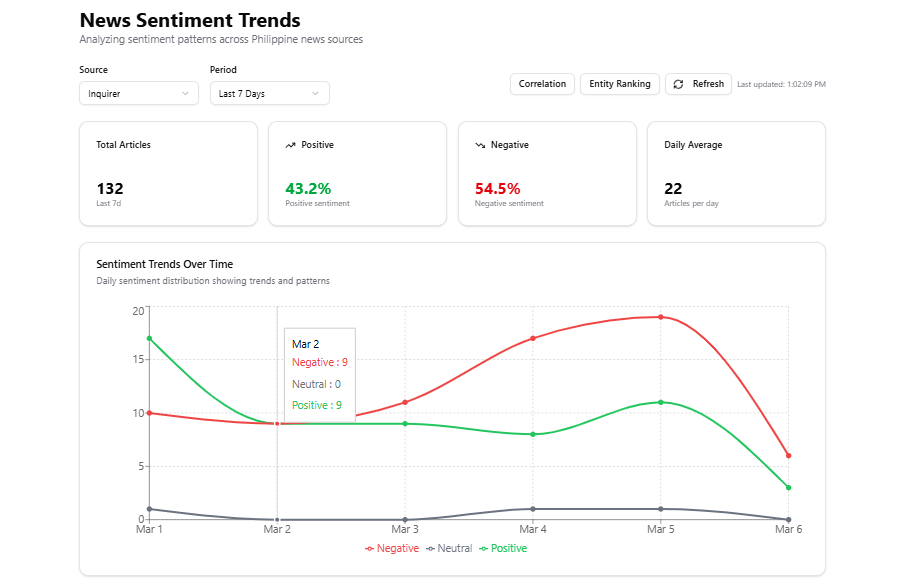
\includegraphics[width=6.26042in,height=4.09375in]{docx-media/1c2657ae7d7803d9ba758bd4fa3ad29899b53d2c.png}

\textbf{Figure 4.6.2 Sentiment Distribution of Rappler Articles}

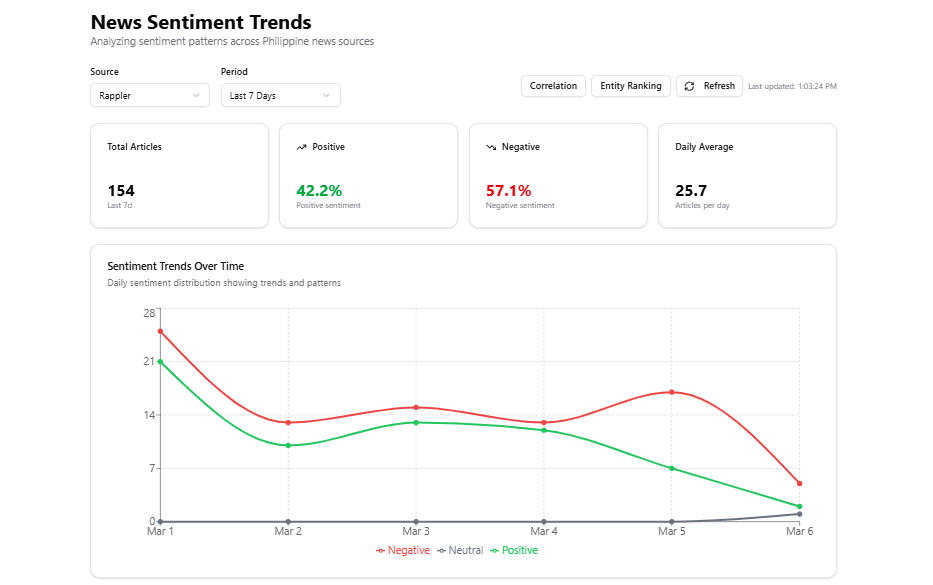
\includegraphics[width=6.26042in,height=3.92708in]{docx-media/3a6996d7e6e6e2eab4d6e23322de63d40d7606fe.png}

\subsubsection{\texorpdfstring{\textbf{Source-Level Sentiment Comparison (Rappler vs. Inquirer)}}{Source-Level Sentiment Comparison (Rappler vs. Inquirer)}}\label{source-level-sentiment-comparison-rappler-vs.-inquirer}

\textbf{Figures 4.6.1 and 4.6.2} presents a source-specific sentiment comparison between \textbf{Rappler} and \textbf{Inquirer} over the same seven-day observation window. By applying the source filter in the Sentiment Trends module, the system isolates articles from individual news outlets and computes sentiment distributions independently.

For \textbf{Inquirer}, the dataset contains \textbf{132 analyzed articles}, with \textbf{43.2\% classified as positive}, \textbf{54.5\% negative}, and a small portion categorized as neutral. The daily timeline shows that negative sentiment becomes more prominent between \textbf{March 3 and March 5}, where the proportion of negatively classified articles exceeds 60\% on several days.

Similarly, \textbf{Rappler} exhibits a slightly stronger negative distribution within the analyzed dataset. Out of \textbf{154 articles}, \textbf{57.1\% were classified as negative} while \textbf{42.2\% were positive}. The timeline indicates that negative sentiment consistently outweighs positive sentiment across most days of the observation period, with the most pronounced imbalance occurring on \textbf{March 5}, where negative articles accounted for more than 70\% of the daily total.

\textbf{Analytics \& Correlation Screen (Comparative View)}

This screen focuses on the statistical alignment between the six news sources. It features the Source Correlation Matrix, a heatmap visualization based on \textbf{Pearson \emph{r} calculations} {[}13, 20{]} of daily sentiment averages. The report measures the strength of the statistical association between source-level sentiment patterns, identifying which outlets exhibit synchronized fluctuations in tone over time. This interface provides a mathematical framework for observing shared trends in the Philippine media landscape.

\textbf{Figure 4.7 Heat Map Source Correlation}

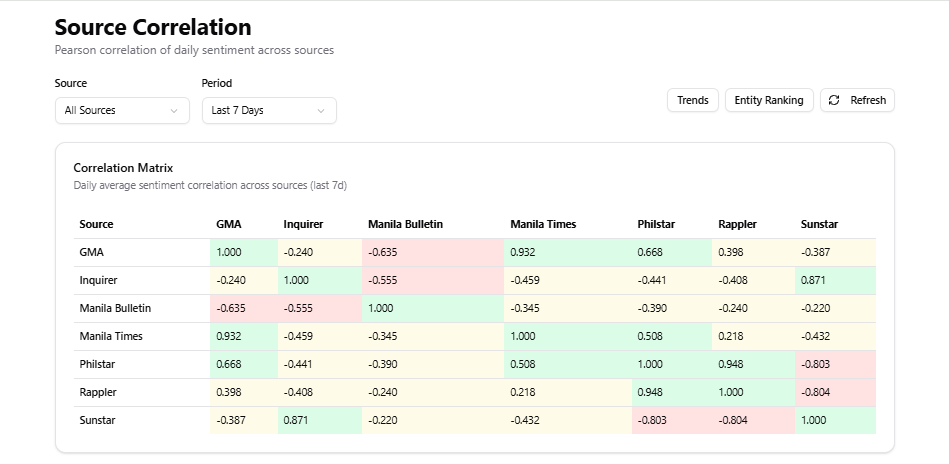
\includegraphics[width=6.26042in,height=3.0625in]{docx-media/e17139834a472e0b03796f557a362814307d4a78.png}

As shown in \textbf{Figure 4.7}, the correlation matrix presents the pairwise Pearson correlation coefficients of daily average sentiment scores across the seven news sources over the past seven days. The values range from −1 to 1, where 1 indicates perfect positive correlation, −1 indicates perfect negative correlation, and 0 indicates no linear association.

The matrix reveals several notable patterns. For instance, \textbf{GMA and Manila Times} exhibit a strong positive correlation of \textbf{0.932}, suggesting that these sources tend to report news with similar sentiment trends during the observed period.

Some correlations may reflect reporting focus or editorial tone. For example, \textbf{Rappler and Philstar} display a high positive correlation (\textbf{0.948}), which could indicate synchronized coverage on certain national events, while \textbf{GMA and Inquirer} show a negative correlation (\textbf{−0.240}), suggesting occasional divergence in reporting sentiment.

It is important to note that these correlations do not imply causation or editorial bias; rather, they provide a quantitative measure of how the sentiment patterns of different sources fluctuate together. This analysis allows researchers to identify clusters of media outlets with similar reporting behavior and to explore patterns in how news sentiment evolves across the Philippine media landscape over time.

\textbf{Figure 4.8 sentiment data and timeline (GMA)}

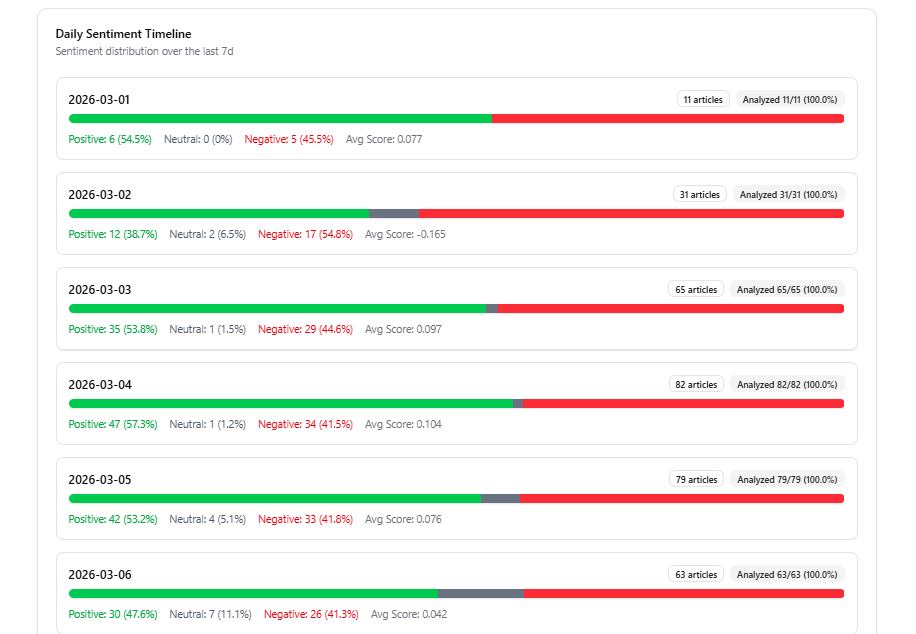
\includegraphics[width=6.26042in,height=4.33333in]{docx-media/249e85845b9ae84eb1ed1e9d76619840b5c4c5d8.png}

\textbf{Figure 4.9 sentiment data and timeline (Manila Times)}

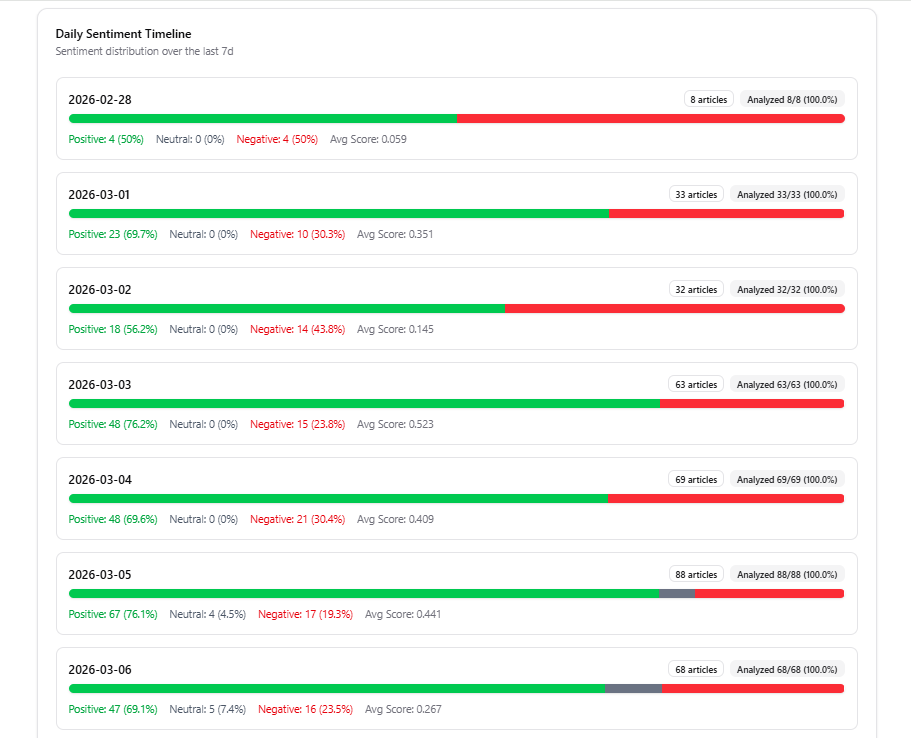
\includegraphics[width=6.26042in,height=5.07292in]{docx-media/400c80febb905ce68baf5a5f1b058d6cb1c76cfc.png}

\textbf{GMA Average Sentiment (see figure 4.8)}

{\def\LTcaptype{none} % do not increment counter
\begin{longtable}[]{@{}
  >{\raggedright\arraybackslash}p{(\linewidth - 2\tabcolsep) * \real{0.5041}}
  >{\raggedright\arraybackslash}p{(\linewidth - 2\tabcolsep) * \real{0.4959}}@{}}
\toprule\noalign{}
\begin{minipage}[b]{\linewidth}\raggedright
\textbf{Date}
\end{minipage} & \begin{minipage}[b]{\linewidth}\raggedright
\textbf{Vader Average Score}
\end{minipage} \\
\midrule\noalign{}
\endhead
\bottomrule\noalign{}
\endlastfoot
March 1 & 0.077 \\
March 2 & -0.165 \\
March 3 & 0.097 \\
March 4 & 0.104 \\
March 5 & 0.076 \\
March 6 & 0.042 \\
\end{longtable}
}

\textbf{Manila Times Average sentiment (see figure 4.9)}

{\def\LTcaptype{none} % do not increment counter
\begin{longtable}[]{@{}
  >{\raggedright\arraybackslash}p{(\linewidth - 2\tabcolsep) * \real{0.4958}}
  >{\raggedright\arraybackslash}p{(\linewidth - 2\tabcolsep) * \real{0.5042}}@{}}
\toprule\noalign{}
\begin{minipage}[b]{\linewidth}\raggedright
\textbf{Date}
\end{minipage} & \begin{minipage}[b]{\linewidth}\raggedright
\textbf{Vader Average Score}
\end{minipage} \\
\midrule\noalign{}
\endhead
\bottomrule\noalign{}
\endlastfoot
March 1 & 0.351 \\
March 2 & 0.145 \\
March 3 & 0.523 \\
March 4 & 0.409 \\
March 5 & 0.441 \\
March 6 & 0.267 \\
\end{longtable}
}

\textbf{Movement Direction Comparison}

{\def\LTcaptype{none} % do not increment counter
\begin{longtable}[]{@{}
  >{\raggedright\arraybackslash}p{(\linewidth - 6\tabcolsep) * \real{0.2500}}
  >{\raggedright\arraybackslash}p{(\linewidth - 6\tabcolsep) * \real{0.2500}}
  >{\raggedright\arraybackslash}p{(\linewidth - 6\tabcolsep) * \real{0.2500}}
  >{\raggedright\arraybackslash}p{(\linewidth - 6\tabcolsep) * \real{0.2500}}@{}}
\toprule\noalign{}
\begin{minipage}[b]{\linewidth}\raggedright
\textbf{Date}
\end{minipage} & \begin{minipage}[b]{\linewidth}\raggedright
\textbf{GMA}
\end{minipage} & \begin{minipage}[b]{\linewidth}\raggedright
\textbf{Manila Times}
\end{minipage} & \begin{minipage}[b]{\linewidth}\raggedright
\textbf{Result}
\end{minipage} \\
\midrule\noalign{}
\endhead
\bottomrule\noalign{}
\endlastfoot
March 1 & ↑ positive score & ↑ positive score & \textbf{match} \\
March 2 & ↓ drop score & ↓ drop score & \textbf{match} \\
March 3 & ↑ rise score & ↑ rise score & \textbf{match} \\
March 4 & ↑ rise score & ↑ rise score & \textbf{match} \\
March 5 & → stable & → stable & \textbf{match} \\
March 6 & ↓ drop score & ↓ drop score & \textbf{match} \\
\end{longtable}
}

\textbf{Relationship Between GMA and Manila Times}

The correlation matrix in \textbf{figure 4.7} reveals a very strong positive relationship between \textbf{GMA and Manila Times (r = 0.932)}. This indicates that the daily sentiment patterns of the two outlets move in a highly synchronized manner during the observation period. Although the overall sentiment distribution differs---where Manila Times exhibits a substantially higher proportion of positive articles \textbf{(70.6\%)} compared to \textbf{GMA (52\%)}, both sources demonstrate similar directional changes in sentiment across the same days. For example, both outlets exhibit a noticeable drop in sentiment on March 2 followed by a consistent rise between \textbf{March 3 and March 4} before stabilizing toward the end of the observation window. This pattern suggests that the outlets may be responding to similar news cycles or events during the period analyzed. However, the correlation should be interpreted strictly as a statistical relationship rather than evidence of editorial alignment or influence.

\textbf{Entity Ranking Screen (Top Mentioned Entities)}

This screen presents the statistical association between prominent news actors and the emotional tone of their coverage. It displays a ranked list of entities (Persons, Organizations, and Geopolitical Entities) paired with their Average Sentiment Score. By cross-referencing mention frequency with sentiment data, this form allows users to observe the prevailing media tone associated with specific entities. This feature provides a quantitative basis for analyzing the representation of various actors across the collected news corpus.

The comparison demonstrates how the system can analyze sentiment trends at the individual source level, enabling researchers to examine differences in tone across news outlets and explore potential relationships between coverage patterns and sentiment classification results.

\textbf{Figure 4.10 Entity rank list}

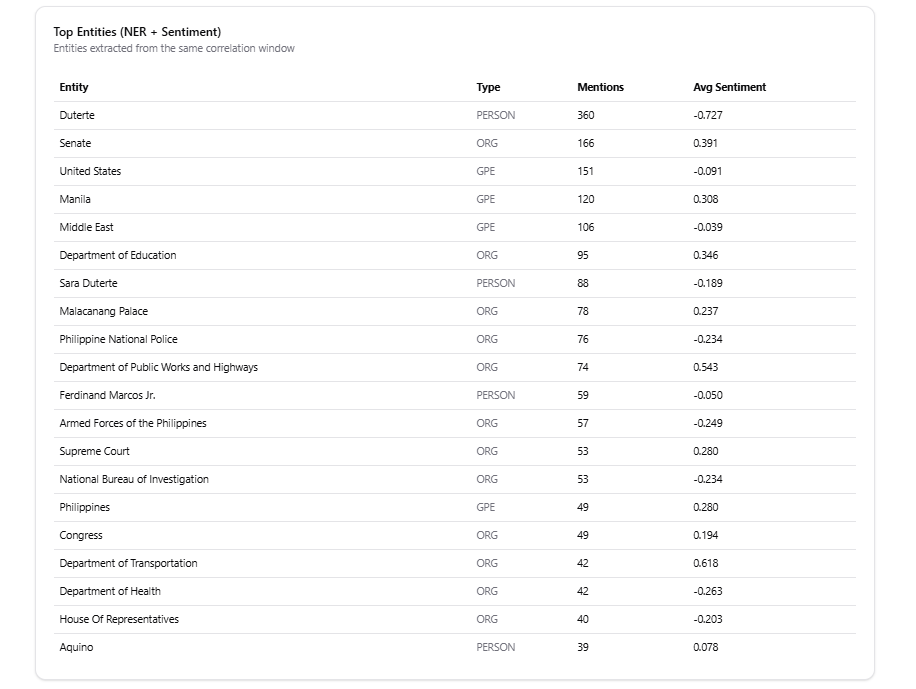
\includegraphics[width=6.26042in,height=4.70833in]{docx-media/a7b3d3db7927b1382a14fe87138960dbed14f84e.png}

The entity ranking results in \textbf{Figure 4.10} reveal that the collected news corpus is dominated by political actors and government institutions. The most frequently mentioned entity is \textbf{Duterte}, appearing 360 times within the analyzed period and exhibiting a strongly negative average sentiment score (-0.727). This pattern likely reflects the prevalence of political or legal developments associated with the figure during the observation window. Other political actors such as \textbf{Sara Duterte} and \textbf{Ferdinand Marcos Jr.} also appear in the ranking, alongside institutional entities including the \textbf{Senate of the Philippines}, \textbf{House of Representatives of the Philippines}, and \textbf{Supreme Court of the Philippines}, indicating that government-related topics form a significant portion of the analyzed news content.

International references are also present in the ranking, such as the \textbf{United States} and the \textbf{Middle East}, indicating that the Philippine news corpus during the observation period included coverage of global geopolitical developments. The sentiment scores associated with these entities are generally close to neutral but slightly negative. This pattern may reflect the nature of international news reporting, which frequently focuses on \textbf{political tensions, security concerns, or conflict-related events}. Overall, the entity ranking demonstrates how the system can quantitatively identify prominent actors within the news dataset while simultaneously associating them with the prevailing sentiment expressed in the articles

\textbf{Source Articles Screen (Per-Source Listing with Search)}

For each news outlet, the system provides a dedicated article listing interface equipped with a high-performance query and filtering mechanism. Considering the substantial volume of data collected, averaging more than 250 articles per day over a four-month period, this search functionality is essential for efficient data discovery and retrieval. Users may conduct keyword-based searches to isolate specific themes such as crime-related reports, political figures including Bongbong Marcos and Rodrigo Duterte, business entities such as Ayala Corporation and San Miguel Corporation, or geographic locations including Iloilo City, Guimaras and the Middle East. The resulting dataset enables researchers to examine the associated sentiment classifications and analyze the frequency of entities within a defined topic or event, thereby supporting more focused and systematic interpretation of media coverage.

\textbf{Figure 4.11 Search result for (Crime)}

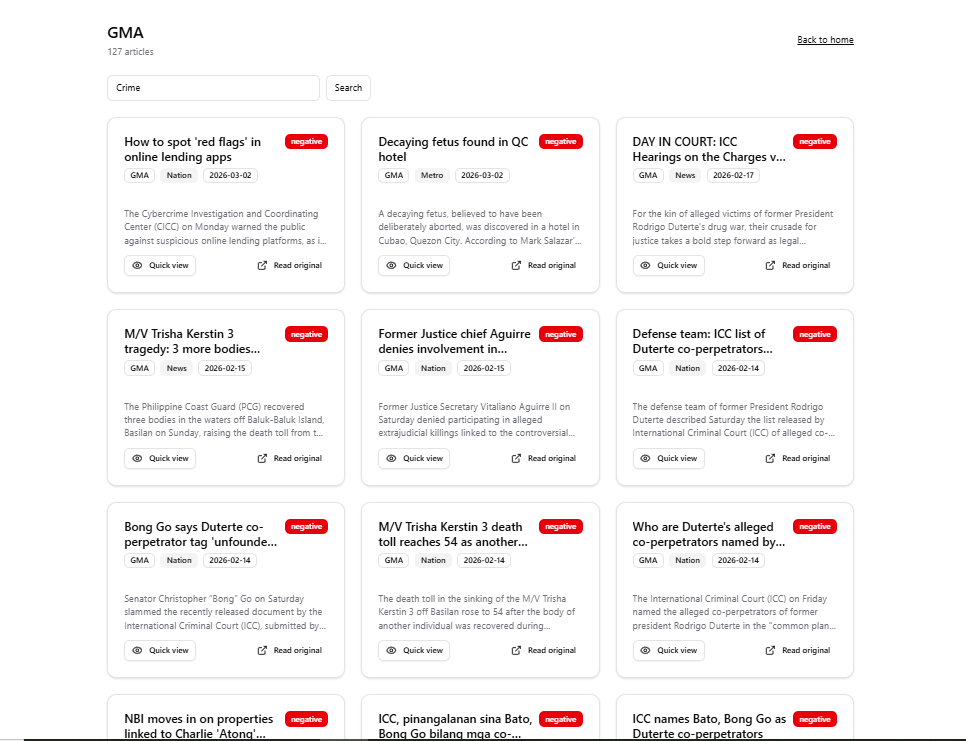
\includegraphics[width=6.26042in,height=4.80208in]{docx-media/3242ca4b5664f3f9fa5933786ca48efa2dedac68.png}

As shown in \textbf{Figure 4.11}, the system provides a query feature that allows users to filter the historical database by keywords. In this example, a search for the keyword \emph{\textbf{``crime''}} was performed across the collected news corpus. The retrieved articles predominantly exhibit Negative sentiment, reflecting the lexicon-based classification patterns of the VADER analyzer for crime-related news, which is consistent with the generally negative nature of crime-related news reporting.

Rather than asserting definitive sentiment accuracy, the results illustrate how the VADER sentiment analyzer categorizes articles containing lexicons typically associated with crime and conflict. The interface enables researchers to examine not only the retrieved articles but also their associated sentiment labels, providing an overview of how sensitive topics are represented in the dataset over a four-month historical period.

\section{\texorpdfstring{\textbf{Article Quick View (Modal Dialog)}}{Article Quick View (Modal Dialog)}}\label{article-quick-view-modal-dialog}

Instead of redirecting users to a separate article detail page, the system provides an in-page ``Quick View'' modal dialog. This modal displays the full article title, metadata (source, publication date, and category), a sentiment label badge, and a preview of the article text. Additionally, a link is included to allow users to open the original article from its official source. This approach improves user experience by minimizing page transitions while preserving access to complete information.

\textbf{Figure 4.12 Quick View Modal}

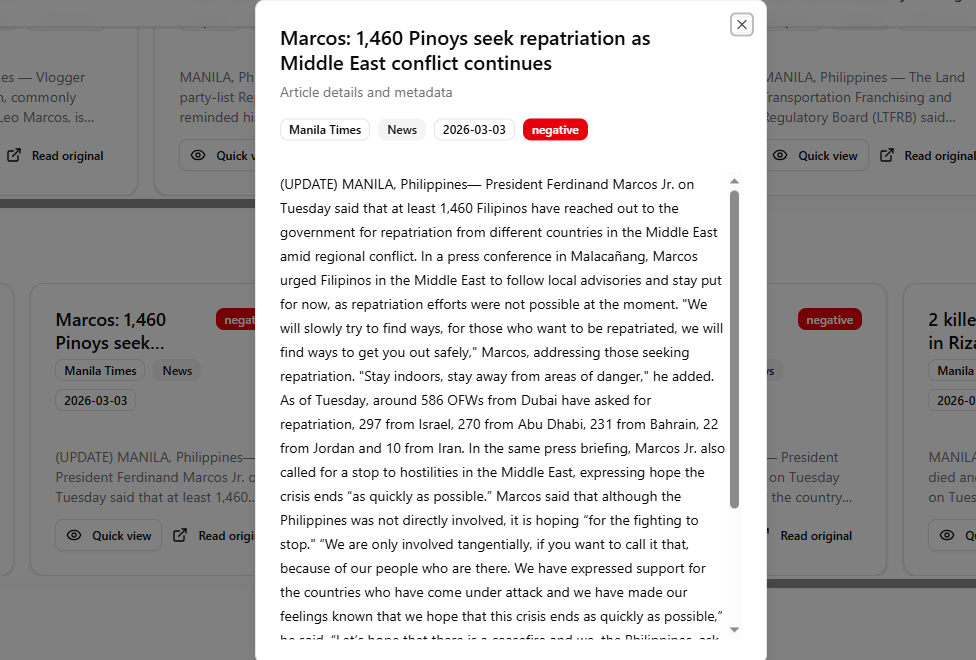
\includegraphics[width=6.26042in,height=3.67857in]{docx-media/401dc19e7445427da9a2bd79b9372b288d0e17d6.png}

\textbf{Reports}

The system generates analytical summaries derived from the processed news dataset. Reports include:

\textbf{Sentiment Trends Report}

This is a longitudinal time-series report that visualizes the fluctuations of positive, neutral, and negative sentiment over a user-defined period. By aggregating daily sentiment data, the report allows researchers to observe shifts in media tone. It includes optional source-level filtering to compare individual outlet trends against the national aggregate.

\textbf{Cross-Platform Sentiment Correlation Matrix}

This report generates a matrix of Pearson correlation coefficients \emph{r} and associated p-values calculated from source-level daily sentiment averages. It measures the statistical association strength between the sentiment patterns of different news outlets. This report provides a mathematical basis for observing synchronized reporting cycles without implying causal influence or intentional bias.

\textbf{Entity-Sentiment Rank and Association Report}

This report presents a ranked list of extracted entities (Persons, Organizations, and GPEs) {[}26{]} paired with their mention frequency and mean sentiment values. Integrated into the correlation module, it allows users to determine the prevailing emotional tone directed toward specific actors within the same analytical timeframe, facilitating a deeper understanding of entity portrayal in the news.

\textbf{Database-Backed Article-Level Audit Records}

The system maintains granular article-level logs within the Supabase relational schema (specifically the articles, analysis, and scraping\_logs tables). These records serve as a technical audit trail used to verify the integrity of visual chart outputs and perform system diagnostics. While not a standalone front-end page, this database-backed capability enables manual validation workflows and ensures the transparency of the automated NLP pipeline.

\textbf{Data Design (Logical Interpretation)}

The system employs a relational data model implemented in PostgreSQL via Supabase {[}6, 19{]}. The design organizes the collected news data, NLP outputs, and operational logs to ensure traceability, consistency, and analytical flexibilit\textbf{y}. Core logical entities, their attributes, and relationships are described below.

\textbf{Core Entities}

{\def\LTcaptype{none} % do not increment counter
\begin{longtable}[]{@{}
  >{\raggedright\arraybackslash}p{(\linewidth - 4\tabcolsep) * \real{0.1747}}
  >{\raggedright\arraybackslash}p{(\linewidth - 4\tabcolsep) * \real{0.3344}}
  >{\raggedright\arraybackslash}p{(\linewidth - 4\tabcolsep) * \real{0.4908}}@{}}
\toprule\noalign{}
\begin{minipage}[b]{\linewidth}\raggedright
\textbf{Entity}
\end{minipage} & \begin{minipage}[b]{\linewidth}\raggedright
\textbf{Attributes}
\end{minipage} & \begin{minipage}[b]{\linewidth}\raggedright
\textbf{Description}
\end{minipage} \\
\midrule\noalign{}
\endhead
\bottomrule\noalign{}
\endlastfoot
\textbf{Source} & Source\_name & Represents each news outlet. Serves as the primary reference for articles and scraping logs. One source may publish multiple articles and have multiple associated scraping runs. \\
\textbf{Article} & Id, source\_name, title, url, published\_at, category & Stores metadata and content of each scraped news article. The id ensures uniqueness, while source\_name links to the corresponding Source. Each Article may have multiple NLP analysis records over time. \\
\textbf{Analysis} & Id, article\_id, model\_type, model\_version, sentiment\_score, sentiment\_label, created\_at & Stores NLP outputs for each article, including sentiment score, sentiment classification, model metadata, and processing timestamps. Multiple entries may exist per article to accommodate repeated or updated analyses. \\
\textbf{Scraping log} & Id, source\_name, status, articles\_scraped, started\_at, completed\_at & Records operational telemetry for each scraping run, including execution status, number of articles collected, and timing. Enables auditing of the data collection process. \\
\textbf{Entity Statistics} & entity\_name, entity\_type, mention\_frequency, average\_sentiment & Aggregated information for Persons, Organizations, and Geopolitical Entities. Generated dynamically from Article and Analysis tables via analytical queries; it is \textbf{not persistently stored} in the database. \\
\end{longtable}
}

\section{Entity Relationship Diagram (Logical Interpretation)}\label{entity-relationship-diagram-logical-interpretation}

\section{\texorpdfstring{\textbf{Figure 4.13} \textbf{Entity Relationship Diagram of the News Sentiment Analysis System}}{Figure 4.13 Entity Relationship Diagram of the News Sentiment Analysis System}}\label{figure-4.13-entity-relationship-diagram-of-the-news-sentiment-analysis-system}

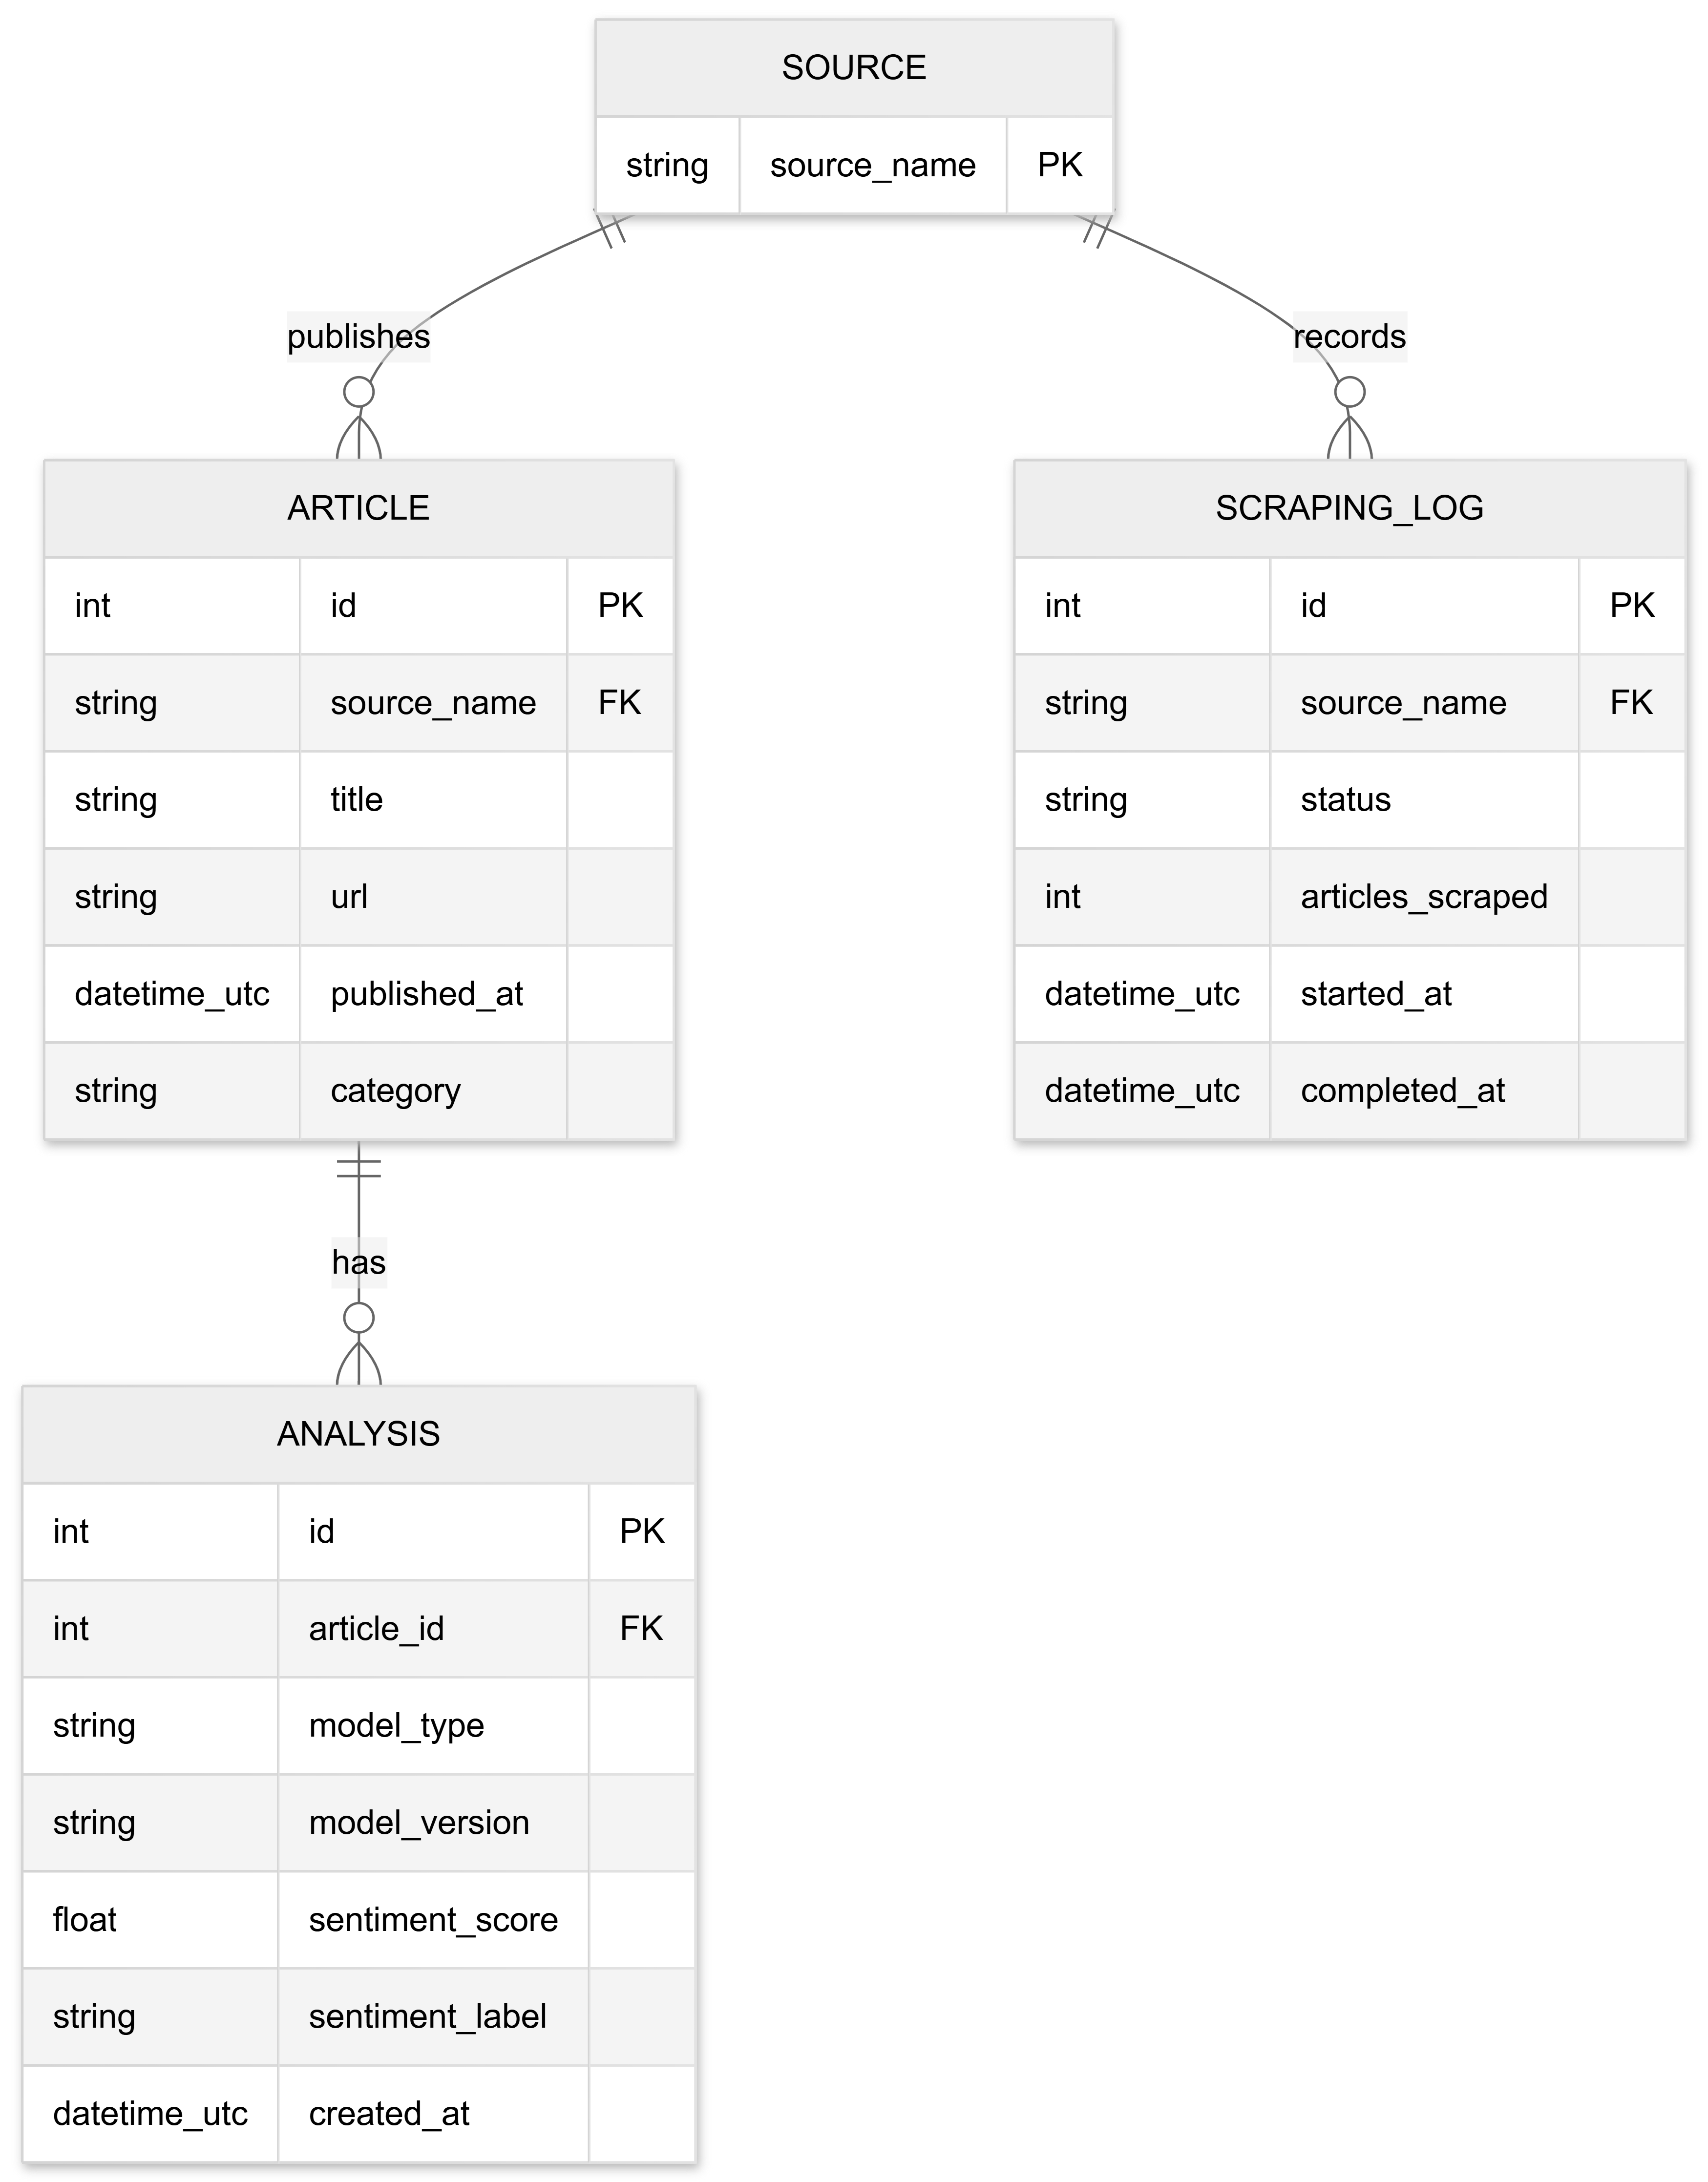
\includegraphics[width=4.89583in,height=6.26042in]{docx-media/4b7c86a7a45af39fc2f8df21f810c186c6d32c3a.png}

\textbf{Figure 4.13} illustrates the system's core logical data model. The SOURCE entity represents each news outlet, while ARTICLE stores the scraped news records collected from these sources. The ANALYSIS entity contains the sentiment analysis outputs generated for each article, and SCRAPING\_LOG records operational telemetry related to scraper executions.

The primary relationships in the model include: a one-to-many relationship between SOURCE and ARTICLE, indicating that each source may publish multiple articles; a one-to-many relationship between ARTICLE and ANALYSIS, allowing each article to have multiple sentiment analysis records; and a one-to-many relationship between SOURCE and SCRAPING\_LOG, which records multiple scraping runs per source.

This separation of entities ensures that raw collected data, NLP analysis outputs, and operational logging are maintained independently. Such a structure improves traceability, supports historical analysis, and enables the system to generate analytical reports including sentiment trends, source correlation, and entity-based statistics.

\textbf{Development}

The development phase implemented the proposed system using a full-stack web architecture consisting of a React-based client interface, a Python-based backend service layer, and a managed relational cloud database. Development followed an iterative build--test--refine workflow, where scraper reliability, sentiment analysis accuracy, and dashboard responsiveness were progressively improved through module-level validation and integration testing.

This phase ensured that each system component---from automated news collection to sentiment analytics visualization---operated reliably within the integrated architecture.

\textbf{Software Specification}

The technical components of the system were selected to support high-speed web scraping and real-time linguistic processing. To ensure transparency and reproducibility, the following specifications were extracted directly from the project's core configuration and dependency files (including backend/Dockerfile, docker-compose.yml, requirements.txt, and package.json).

{\def\LTcaptype{none} % do not increment counter
\begin{longtable}[]{@{}
  >{\raggedright\arraybackslash}p{(\linewidth - 6\tabcolsep) * \real{0.2267}}
  >{\raggedright\arraybackslash}p{(\linewidth - 6\tabcolsep) * \real{0.3002}}
  >{\raggedright\arraybackslash}p{(\linewidth - 6\tabcolsep) * \real{0.3226}}
  >{\raggedright\arraybackslash}p{(\linewidth - 6\tabcolsep) * \real{0.1505}}@{}}
\toprule\noalign{}
\begin{minipage}[b]{\linewidth}\raggedright
\textbf{Software / Tool}
\end{minipage} & \begin{minipage}[b]{\linewidth}\raggedright
\textbf{Version (from project)}
\end{minipage} & \begin{minipage}[b]{\linewidth}\raggedright
\textbf{Purpose}
\end{minipage} & \begin{minipage}[b]{\linewidth}\raggedright
\textbf{Reference}
\end{minipage} \\
\midrule\noalign{}
\endhead
\bottomrule\noalign{}
\endlastfoot
\textbf{Operating System (Host)} & Windows 10/11, MacOS Sonoma & Local development environment & --- \\
\textbf{Python (Host)} & 3.14.2 & Local scripting/testing environment & {[}37{]} \\
\textbf{Node.js} & v24.13.0 & Frontend runtime/tooling & {[}38{]} \\
\textbf{npm} & 11.6.2 & Package management/build scripts & {[}40{]} \\
\textbf{Frontend Framework} & Next.js 15.5.2 & Web UI and routing & {[}31{]} \\
\textbf{UI Runtime} & React 19.1.0 + React DOM & Component-based frontend rendering & {[}32{]} \\
\textbf{Styling} & Tailwind CSS 4 & Utility-first frontend styling & {[}33{]} \\
\textbf{Charts} & Recharts 3.2.0 & Trends/correlation visualizations & {[}34{]} \\
\textbf{Frontend Data Client} & @supabase/supabase-js 2.56.1 & Supabase access from frontend & {[}19{]} \\
\textbf{Backend Framework} & FastAPI 0.104.1 & REST API endpoints & {[}27{]} \\
\textbf{ASGI Server} & Uvicorn 0.30.1 & Backend app serving & {[}28{]} \\
\textbf{Task Queue/ Scheduler} & Celery Beat + celery-redbeat & Tasker/Async scraping/analysis jobs & {[}29{]} \\
\textbf{Queue/Cache} & Redis 7 (image), redis-py 5.0.4 & Broker + caching & {[}15{]} \\
\textbf{Database} & Supabase (PostgreSQL) & Persistent relational storage & {[}6, 19{]} \\
\textbf{Python Supabase Client} & supabase 2.6.0 & Backend DB access & {[}19{]} \\
\textbf{Scraping HTTP} & httpx 0.27.0, requests 2.31.0 & Network fetches & {[}41{]} \\
\textbf{HTML Parsing} & beautifulsoup4 4.12.3, lxml & Article parsing/cleanup & {[}39{]} \\
\textbf{Browser Automation} & Playwright 1.46.0 & Dynamic/anti-bot scraping & {[}30{]} \\
\textbf{Sentiment NLP} & NLTK 3.8.1 (VADER) & Sentiment scoring & {[}1, 8{]} \\
\textbf{NER NLP} & spaCy 3.7.4 & Entity extraction & {[}26{]} \\
\textbf{Stats/Math} & NumPy, SciPy, Pandas, scikit-learn & Correlation/statistical analytics & {[}7, 13{]}, {[}20{]}, {[}36{]} \\
\textbf{Containerization} & Docker + Docker Compose & Service orchestration & {[}35{]} \\
\end{longtable}
}

\textbf{Hardware Specification}

The development and evaluation setup used a consumer-grade machine:

\begin{enumerate}
\def\labelenumi{\arabic{enumi}.}
\item
  CPU: Intel Core i5 (8th Generation).
\item
  Memory: 16 GB RAM.
\item
  GPU: Integrated graphics (no dedicated GPU required for current NLP pipeline).
\item
  Storage: SSD/HDD with sufficient space for dataset growth and logs.
\item
  Network: Stable internet connection for scraping and cloud database access.
\end{enumerate}

This hardware configuration was sufficient for development, testing, and evaluation of the proposed system. The system relies on lexicon-based sentiment analysis rather than computationally intensive deep learning models, allowing the analysis pipeline to operate efficiently on consumer-grade hardware.

\textbf{Program Specification}

The program is organized into coordinated modules:

\begin{enumerate}
\def\labelenumi{\arabic{enumi}.}
\item
  Scraping Module: Collects articles from supported news sources, normalizes fields, and handles retries/timeouts.
\item
  Deduplication and Storage Module: Prevents duplicate insertion and writes validated records into articles.
\item
  Sentiment Analysis Module: Processes article text using long-form weighted VADER and stores outputs in analysis (model\_type=sentiment).
\item
  Entity Mining Module: Extracts entities (PERSON/ORG/GPE) and supports ranking and association analytics.
\item
  Analytics API Module: Produces trend timelines, source correlation matrix, and entity-focused reports.
\item
  UI Rendering Module: Presents dashboard cards, trend charts, correlation matrix, and searchable source pages.
\end{enumerate}

\textbf{Programming Environment}

\textbf{Front End}

The front-end interface of the system was developed using \textbf{Next.js {[}31{]}}, a React-based web framework that enables efficient component-based interface development and server-side rendering capabilities. The application was implemented using \textbf{TypeScript} to improve type safety and maintain code reliability.

For styling and layout, \textbf{Tailwind CSS {[}33{]}} was used to provide a responsive and utility-first design framework. UI components were implemented using the \textbf{shadcn/ui component library}, which provides reusable and accessible interface elements built on top of \textbf{React {[}32{]}} and Radix UI primitives.

Data visualization components used in the dashboard---including sentiment trend charts and correlation visualizations---were implemented using the \textbf{Recharts charting library {[}34{]}}, which integrates seamlessly with React applications and enables dynamic rendering of statistical data.

\textbf{Back End}

The back-end services of the system were implemented using \textbf{FastAPI {[}27{]}}, a Python-based web framework designed for high-performance API development. FastAPI provides asynchronous request handling and efficient data serialization, enabling the system to support real-time analytics queries from the dashboard interface.

Background processing tasks such as automated scraping and sentiment analysis were executed using \textbf{Celery {[}29{]}}, a distributed task queue system. Celery Beat was used to schedule periodic scraping jobs that continuously collect news articles from supported sources.

\textbf{Redis {[}15{]}} served as the task broker and caching layer for Celery workers, ensuring efficient job distribution and improved response performance.

Persistent data storage was handled by \textbf{Supabase {[}19{]}}, which provides a managed \textbf{PostgreSQL {[}6{]}} database environment.

To ensure consistent deployment and environment isolation, the application services were containerized using \textbf{Docker {[}35{]}}, with Docker Compose used to orchestrate the API server, background workers, and supporting services during development and testing.

\section{\texorpdfstring{\textbf{System Architecture Overview}}{System Architecture Overview}}\label{system-architecture-overview}

\section{The implemented system follows a modular full-stack architecture designed to support automated data collection, natural language processing, and interactive analytics visualization. The architecture consists of four primary layers: data acquisition, processing, storage, and presentation. This layered design enables separation of concerns while supporting scalable processing of news article data.}\label{the-implemented-system-follows-a-modular-full-stack-architecture-designed-to-support-automated-data-collection-natural-language-processing-and-interactive-analytics-visualization.-the-architecture-consists-of-four-primary-layers-data-acquisition-processing-storage-and-presentation.-this-layered-design-enables-separation-of-concerns-while-supporting-scalable-processing-of-news-article-data.}

The \textbf{data acquisition layer} is responsible for collecting news articles from supported Philippine news sources through automated scraping routines. Scraper jobs are executed asynchronously using scheduled background tasks, ensuring that article collection occurs regularly without interrupting the main application services. The scraping mechanism utilizes browser automation through Playwright {[}30{]} to extract article content and metadata from dynamically rendered news pages.

The \textbf{processing layer} performs natural language processing operations on the collected articles. This includes sentiment classification using the VADER sentiment analyzer {[}8{]} and entity extraction using spaCy's Named Entity Recognition (NER) pipeline {[}26{]}. The processing tasks are executed by distributed worker processes managed by Celery {[}29{]}, enabling parallel handling of article analysis workloads. The task queue is coordinated through Redis {[}15{]}, which functions as the message broker for distributing background processing jobs.

The \textbf{data storage layer} utilizes a PostgreSQL relational database {[}6{]} hosted on Supabase {[}19{]}. This layer stores the scraped article records, sentiment analysis outputs, and operational scraping logs. The relational schema supports structured querying and enables efficient generation of analytical reports such as sentiment timelines, entity frequency distributions, and cross-source sentiment correlation matrices.

The \textbf{presentation layer} is implemented as a web application built using Next.js {[}31{]} and React {[}32{]}, with styling provided through Tailwind CSS {[}33{]}. Data visualization components, including sentiment trend charts and statistical dashboards, are rendered using the Recharts visualization library {[}34{]}. This interface provides interactive dashboards that allow users to explore sentiment trends, compare media sources, and analyze entity-level sentiment patterns within the collected news dataset.

Together, these layers form a scalable data processing pipeline that enables automated news monitoring while maintaining clear separation between data collection, analysis, storage, and visualization components.

\subsection{\texorpdfstring{\textbf{Conclusions}}{Conclusions}}\label{conclusions}

The study successfully designed and implemented an \textbf{Automated Media Sentiment Monitoring System} for Philippine online news sources. The system integrates automated web scraping, natural language processing, and interactive analytics to collect, process, and analyze news articles from multiple media outlets.

The developed platform is capable of automatically gathering news content, performing sentiment classification using the VADER sentiment analyzer, and extracting key named entities from the collected articles. The processed information is then presented through interactive analytical views that enable users to observe sentiment trends over time, compare sentiment patterns across news sources, and identify frequently mentioned entities within the news corpus.

Additional analytical components, including cross-source sentiment correlation and entity--sentiment association, demonstrate how statistical analysis and text mining techniques can be used to explore relationships within large-scale news datasets. The system also maintains database-backed audit records, ensuring traceability through article metadata, sentiment analysis outputs, and scraping logs.

Overall, the system achieved its primary objective of providing an operational platform for automated monitoring and analysis of sentiment patterns in Philippine news media.

\subsection{\texorpdfstring{\textbf{Recommendations}}{Recommendations}}\label{recommendations}

Future improvements may enhance the analytical capabilities, accuracy, and scalability of the proposed system.

\textbf{First}, the development of a manually labeled Philippine news sentiment benchmark dataset is recommended to enable objective evaluation of sentiment classification performance and to calibrate decision thresholds for local linguistic contexts.

\textbf{Second}, improvements in entity normalization techniques may help reduce ambiguity in extracted entity names, particularly for acronyms, aliases, and variations of geopolitical entities.

Third, the implementation of periodic data quality audit\textbf{s} is recommended to ensure the completeness and consistency of scraped news articles across all supported sources.

\textbf{Finally}, future studies may explore the integration of transformer-based natural language \textbf{processing models} as an optional high-accuracy analysis mode. Such models may improve sentiment detection in complex linguistic scenarios while maintaining lexicon-based methods like VADER for environments with limited computational resources.

Future versions of the system may also incorporate topic filtering mechanisms to exclude non-policy news categories such as sports, entertainment, and lifestyle content. Restricting the dataset to policy-relevant domains such as politics, governance, and economics may improve the interpretability of sentiment trends and reduce noise in the analysis.

\textbf{Bibliography}

{[}1{]}

\begin{quote}
Steven Bird, Ewan Klein, and Edward Loper. 2009. \emph{Natural language processing with Python}. O'Reilly, Cambridge.
\end{quote}

{[}2{]}

\begin{quote}
Jan Christian Blaise Cruz and Charibeth Cheng. 2020. Establishing Baselines for Text Classification in Low-Resource Languages. \url{https://doi.org/10.48550/arXiv.2005.02068}
\end{quote}

{[}3{]}

\begin{quote}
Manuel Jr Diaz. 2021. Sentiment Polarity Identification in Banner Headlines of Broadsheets in the Philippines. \emph{Asian J. Media Commun} 5, 2 (December 2021). \url{https://doi.org/10.20885/asjmc.vol5.iss2.art1}
\end{quote}

{[}4{]}

\begin{quote}
Robert M. Entman. 1993. Framing: Toward Clarification of a Fractured Paradigm. \emph{Journal of Communication} 43, 4 (December 1993), 51--58. \url{https://doi.org/10.1111/j.1460-2466.1993.tb01304.x}
\end{quote}

{[}5{]}

\begin{quote}
Manuel B. Garcia. 2020. Sentiment Analysis of Tweets on Coronavirus Disease 2019 (COVID-19) Pandemic from Metro Manila, Philippines. \emph{Cybernetics and Information Technologies} (2020). Retrieved March 13, 2026 from \url{https://manuelgarcia.info/publication/coronavirus-sentiment-analysis-philippines}
\end{quote}

{[}6{]}

\begin{quote}
PostgreSQL Global Development Group. 2026. PostgreSQL. \emph{PostgreSQL}. Retrieved March 14, 2026 from \url{https://www.postgresql.org/}
\end{quote}

{[}7{]}

\begin{quote}
Charles R. Harris, K. Jarrod Millman, Stéfan J. Van Der Walt, Ralf Gommers, Pauli Virtanen, David Cournapeau, Eric Wieser, Julian Taylor, Sebastian Berg, Nathaniel J. Smith, Robert Kern, Matti Picus, Stephan Hoyer, Marten H. Van Kerkwijk, Matthew Brett, Allan Haldane, Jaime Fernández Del Río, Mark Wiebe, Pearu Peterson, Pierre Gérard-Marchant, Kevin Sheppard, Tyler Reddy, Warren Weckesser, Hameer Abbasi, Christoph Gohlke, and Travis E. Oliphant. 2020. Array programming with NumPy. \emph{Nature} 585, 7825 (September 2020), 357--362. \url{https://doi.org/10.1038/s41586-020-2649-2}
\end{quote}

{[}8{]}

\begin{quote}
C. Hutto and Eric Gilbert. 2014. VADER: A Parsimonious Rule-Based Model for Sentiment Analysis of Social Media Text. \emph{ICWSM} 8, 1 (May 2014), 216--225. \url{https://doi.org/10.1609/icwsm.v8i1.14550}
\end{quote}

{[}9{]}

\begin{quote}
S. Kiritchenko, X. Zhu, and S. M. Mohammad. 2014. Sentiment Analysis of Short Informal Texts. \emph{jair} 50, (August 2014), 723--762. \url{https://doi.org/10.1613/jair.4272}
\end{quote}

{[}10{]}

\begin{quote}
Maikel Leon. 2025. From Lexicons to Transformers: An AI View of Sentiment Analysis. \emph{Journal of Intelligent Communication} 4, 2 (September 2025), 13--25. \url{https://doi.org/10.54963/jic.v4i2.1434}
\end{quote}

{[}11{]}

\begin{quote}
Maxwell E. McCombs and Donald L. Shaw. 1972. The Agenda-Setting Function of Mass Media. \emph{Public Opinion Quarterly} 36, 2 (1972), 176. \url{https://doi.org/10.1086/267990}
\end{quote}

{[}12{]}

\begin{quote}
Margaret Mitchell, Jacqui Aguilar, Theresa Wilson, and Benjamin Van Durme. 2013. Open Domain Targeted Sentiment. In \emph{Proceedings of the 2013 Conference on Empirical Methods in Natural Language Processing}, October 2013. Association for Computational Linguistics, Seattle, Washington, USA, 1643--1654. Retrieved March 13, 2026 from \url{https://aclanthology.org/D13-1171/}
\end{quote}

{[}13{]}

\begin{quote}
Fabian Pedregosa, Gaël Varoquaux, Alexandre Gramfort, Vincent Michel, Bertrand Thirion, Olivier Grisel, Mathieu Blondel, Peter Prettenhofer, Ron Weiss, Vincent Dubourg, Jake Vanderplas, Alexandre Passos, David Cournapeau, Matthieu Brucher, Matthieu Perrot, and Édouard Duchesnay. 2011. Scikit-learn: Machine Learning in Python. \emph{Journal of Machine Learning Research} 12, 85 (2011), 2825--2830. Retrieved March 13, 2026 from \url{http://jmlr.org/papers/v12/pedregosa11a.html}
\end{quote}

{[}14{]}

\begin{quote}
Neha Rana. 2025. Lexicon vs. Transformer-Based Models for Sentiment Analysis. \emph{Medium}. Retrieved March 14, 2026 from \url{https://rananeha.medium.com/lexicon-vs-transformer-based-models-for-sentiment-analysis-56a80c8f4b10}
\end{quote}

{[}15{]}

\begin{quote}
Redis. Redis - The Real-time Data Platform. \emph{Redis}. Retrieved March 14, 2026 from \url{https://redis.io/}
\end{quote}

{[}16{]}

\begin{quote}
Stuart Soroka, Patrick Fournier, and Lilach Nir. 2019. Cross-national evidence of a negativity bias in psychophysiological reactions to news. \emph{Proc. Natl. Acad. Sci. U.S.A.} 116, 38 (September 2019), 18888--18892. \url{https://doi.org/10.1073/pnas.1908369116}
\end{quote}

{[}17{]}

\begin{quote}
CMFR Staff. 2022. MEDIA AND ELECTIONS 2022. \emph{CMFR}. Retrieved March 13, 2026 from \url{https://cmfr-phil.org/elections-2022/media-and-elections-2022/}
\end{quote}

{[}18{]}

\begin{quote}
Martina Stockhause and Michael Lautenschlager. 2018. \emph{Ddc Report 2017 Of Wdcc}. Zenodo. \url{https://doi.org/10.5281/ZENODO.1212314}
\end{quote}

{[}19{]}

\begin{quote}
Supabase. 2026. Supabase Docs. Retrieved March 14, 2026 from \url{https://supabase.com/docs}
\end{quote}

{[}20{]}

\begin{quote}
Pauli Virtanen, Ralf Gommers, Travis E. Oliphant, Matt Haberland, Tyler Reddy, David Cournapeau, Evgeni Burovski, Pearu Peterson, Warren Weckesser, Jonathan Bright, Stéfan J. Van Der Walt, Matthew Brett, Joshua Wilson, K. Jarrod Millman, Nikolay Mayorov, Andrew R. J. Nelson, Eric Jones, Robert Kern, Eric Larson, C J Carey, İlhan Polat, Yu Feng, Eric W. Moore, Jake VanderPlas, Denis Laxalde, Josef Perktold, Robert Cimrman, Ian Henriksen, E. A. Quintero, Charles R. Harris, Anne M. Archibald, Antônio H. Ribeiro, Fabian Pedregosa, Paul Van Mulbregt, SciPy 1.0 Contributors, Aditya Vijaykumar, Alessandro Pietro Bardelli, Alex Rothberg, Andreas Hilboll, Andreas Kloeckner, Anthony Scopatz, Antony Lee, Ariel Rokem, C. Nathan Woods, Chad Fulton, Charles Masson, Christian Häggström, Clark Fitzgerald, David A. Nicholson, David R. Hagen, Dmitrii V. Pasechnik, Emanuele Olivetti, Eric Martin, Eric Wieser, Fabrice Silva, Felix Lenders, Florian Wilhelm, G. Young, Gavin A. Price, Gert-Ludwig Ingold, Gregory E. Allen, Gregory R. Lee, Hervé Audren, Irvin Probst, Jörg P. Dietrich, Jacob Silterra, James T Webber, Janko Slavič, Joel Nothman, Johannes Buchner, Johannes Kulick, Johannes L. Schönberger, José Vinícius De Miranda Cardoso, Joscha Reimer, Joseph Harrington, Juan Luis Cano Rodríguez, Juan Nunez-Iglesias, Justin Kuczynski, Kevin Tritz, Martin Thoma, Matthew Newville, Matthias Kümmerer, Maximilian Bolingbroke, Michael Tartre, Mikhail Pak, Nathaniel J. Smith, Nikolai Nowaczyk, Nikolay Shebanov, Oleksandr Pavlyk, Per A. Brodtkorb, Perry Lee, Robert T. McGibbon, Roman Feldbauer, Sam Lewis, Sam Tygier, Scott Sievert, Sebastiano Vigna, Stefan Peterson, Surhud More, Tadeusz Pudlik, Takuya Oshima, Thomas J. Pingel, Thomas P. Robitaille, Thomas Spura, Thouis R. Jones, Tim Cera, Tim Leslie, Tiziano Zito, Tom Krauss, Utkarsh Upadhyay, Yaroslav O. Halchenko, and Yoshiki Vázquez-Baeza. 2020. SciPy 1.0: fundamental algorithms for scientific computing in Python. \emph{Nat Methods} 17, 3 (March 2020), 261--272. \url{https://doi.org/10.1038/s41592-019-0686-2}
\end{quote}

{[}21{]}

\begin{quote}
2025. Digital 2025: The Philippines. \emph{DataReportal -- Global Digital Insights}. Retrieved March 13, 2026 from \url{https://datareportal.com/reports/digital-2025-philippines}
\end{quote}

{[}22{]}

\begin{quote}
2025. Data science in central banking: enhancing the access to and sharing of data. (May 2025). Retrieved March 13, 2026 from \url{https://www.bis.org/ifc/publ/ifcb64.pdf}
\end{quote}

{[}23{]}

\begin{quote}
Fake news detection in Philippine news corpus using LDA and sentiment analysis with machine learning \textbar{} Proceedings of the Samahang Pisika ng Pilipinas. Retrieved March 13, 2026 from \url{https://proceedings.spp-online.org/article/view/SPP-2023-PB-40}
\end{quote}

{[}24{]}

\begin{quote}
Media Ownership Monitor Philippines 2023. \emph{Media Ownership Monitor}. Retrieved March 13, 2026 from \url{https://philippines.mom-gmr.org/en/}
\end{quote}

{[}25{]}

\begin{quote}
Like, Comment, and Share: Analyzing Public Sentiments of Government Policies in Social Media. Retrieved March 13, 2026 from \url{http://www.pids.gov.ph/publication/discussion-papers/like-comment-and-share-analyzing-public-sentiments-of-government-policies-in-social-media}
\end{quote}

{[}26{]}

\begin{quote}
Facts \& Figures · spaCy Usage Documentation. \emph{Facts \& Figures}. Retrieved March 13, 2026 from \url{https://spacy.io/usage/facts-figures}
\end{quote}

{[}27{]}

\begin{quote}
FastAPI. Retrieved March 14, 2026 from \url{https://fastapi.tiangolo.com/}
\end{quote}

{[}28{]}

\begin{quote}
Uvicorn. Retrieved March 14, 2026 from \url{https://www.uvicorn.org/}
\end{quote}

{[}29{]}

\begin{quote}
Celery - Distributed Task Queue --- Celery 5.6.2 documentation. Retrieved March 14, 2026 from \url{https://docs.celeryq.dev/en/stable/}
\end{quote}

{[}30{]}

\begin{quote}
Fast and reliable end-to-end testing for modern web apps \textbar{} Playwright. Retrieved March 14, 2026 from \url{https://playwright.dev/}
\end{quote}

{[}31{]}

\begin{quote}
Next.js by Vercel - The React Framework. Retrieved March 14, 2026 from \url{https://nextjs.org/}
\end{quote}

{[}32{]}

\begin{quote}
React. Retrieved March 14, 2026 from \url{https://react.dev/}
\end{quote}

{[}33{]}

\begin{quote}
Tailwind CSS - Rapidly build modern websites without ever leaving your HTML. Retrieved March 14, 2026 from \url{https://tailwindcss.com/}
\end{quote}

{[}34{]}

\begin{quote}
Recharts. Retrieved March 14, 2026 from \url{https://recharts.github.io/}
\end{quote}

{[}35{]}

\begin{quote}
Docker: Lightweight Linux Containers for Consistent Development and Deployment \textbar{} Linux Journal. Retrieved March 14, 2026 from \url{https://www.linuxjournal.com/content/docker-lightweight-linux-containers-consistent-development-and-deployment}
\end{quote}

{[}36{]}

\begin{quote}
Wes McKinney. \emph{Wes McKinney}. Retrieved March 14, 2026 from \url{https://wesmckinney.com/static/pandas_scipy_2010.pdf}
\end{quote}
